\documentclass{wileySix}

\usepackage{graphicx}
\usepackage{listings}

\usepackage{color}

\definecolor{codegreen}{rgb}{0,0.6,0}
\definecolor{codegray}{rgb}{0.5,0.5,0.5}
\definecolor{codepurple}{rgb}{0.58,0,0.82}
\definecolor{backcolour}{rgb}{0.95,0.95,0.92}

\lstdefinestyle{mystyle}{
    backgroundcolor=\color{backcolour},
    commentstyle=\color{codegreen},
    keywordstyle=\color{magenta},
    numberstyle=\tiny\color{codegray},
    stringstyle=\color{codepurple},
    basicstyle=\footnotesize,
    breakatwhitespace=false,
    breaklines=true,
    captionpos=b,
    keepspaces=true,
    numbers=left,
    numbersep=5pt,
    showspaces=false,
    showstringspaces=false,
    showtabs=false,
    tabsize=2,
    language=TeX,
	caption=Coy kasih caption dong,
	label={lstlisting_nya_ada_yang_belum_dikasih_label}
}

\lstset{style=mystyle}

\usepackage{w-bookps}

\setcounter{secnumdepth}{3}

\setcounter{tocdepth}{2}


\docropmarks


\newcommand{\VT}[1]{\ensuremath{{V_{T#1}}}}


\newbox\sectsavebox
\setbox\sectsavebox=\hbox{\boldmath\VT{xyz}}



\begin{document}


\booktitle{Loogbok AS}
\subtitle{Dalam 24 Jam}

\authors{Etika Khusnul Laeli, Jenly Ramdan\\
\affil{D4 Informatics Engineering}}

\offprintinfo{Cerdas Menguasai Android Studio, First Edition}{Etika Khusnul Laeli, Jnely Ramdan}


\halftitlepage

\titlepage


\begin{copyrightpage}{2020}
%Survey Methodology / Robert M. Groves . . . [et al.].
%\       p. cm.---(Wiley series in survey methodology)
%\    ``Wiley-Interscience."
%\    Includes bibliographical references and index.
%\    ISBN 0-471-48348-6 (pbk.)
%\    1. Surveys---Methodology.  2. Social 
%\  sciences---Research---Statistical methods.  I. Groves, Robert M.  II. %
%Series.\\
%
%HA31.2.S873 2007
%001.4'33---dc22                                             2004044064
\end{copyrightpage}

\dedication{`Jika Kamu tidak dapat menahan lelahnya belajar,
Maka kamu harus sanggup menahan perihnya Kebodohan.'
~Imam Syafi'i~}

\begin{contributors}
\name{Etika Khusnul Laeli, Jenly Ramdan} D4 Informatics Engineering ., Politeknik Pos Indonesia, Bandung,
Indonesia



\end{contributors}

\contentsinbrief
\tableofcontents
\listoffigures
\listoftables
\lstlistoflistings


\begin{foreword}
Sepatah kata dari Kaprodi, Kabag Kemahasiswaan dan Mahasiswa
\end{foreword}

\begin{preface}
Buku ini diciptakan bagi yang awam dengan Aplikasi Android sekalipun.

\prefaceauthor{Etika Khusnul Laeli , Jenly Ramdan}
\where{Bandung, Jawa Barat\\
Januari, 2020}
\end{preface}


\begin{acknowledgments}
Terima kasih atas semua masukan dari para dosen pembimbing, mahasiswa/i agar bisa membuat buku ini 
lebih baik dan lebih mudah dimengerti.

Terima kasih ini juga ditujukan khusus untuk kedua orang tua yang selalu mensupport dan mendoakan kami yang 
telah fokus untuk belajar dan memahami bagaimana buku ini mendampingi proses Proyek 2.
\authorinitials{Etika Khusnul Laeli, Jenly Ramdan}
\end{acknowledgments}

\begin{acronyms}
\acro{ACGIH}{American Conference of Governmental Industrial Hygienists}
\acro{AEC}{Atomic Energy Commission}
\acro{OSHA}{Occupational Health and Safety Commission}
\acro{SAMA}{Scientific Apparatus Makers Association}
\acro{EPS}{Encapsulated PostScript}
\acro{HTBP}{Here Tab Bottom Paragraph}
\acro{IDE}{Integrated Development Environment}
\acro{GPL}{General Public Lisence}
\end{acronyms}

\begin{glossary}
\term{Android Studio}adalah Lingkungan Pengembangan Terpadu(Integrated Development Environment/IDE), yang didasarkan pada IntelliJ IDEA.

\term{Android SDK Build-Tools} 
Wajib. Mencakup fitur untuk membuat aplikasi Android. 

\term{Android SDK Platform-Tools} 
Wajib. Mencakup berbagai fitur yang diperlukan oleh platform Android, termasuk fitur adb.

\term {Android SDK Tools} 
Wajib. Mencakup fitur penting seperti ProGuard.

\term {Android Emulator} Direkomendasikan. Fitur emulasi perangkat berbasis QEMU yang dapat Anda gunakan untuk men-debug dan menguji aplikasi di lingkungan runtime Android sebenermya.

\term {Android SDK Plaform}
 Wajib. Lingkungan Anda memerlukan setidaknya satu platform agar aplikasi dapat dikompilasi.

\term {Image Sistem Inel atau ARM} Direkomendasikan. Image sisem diperlukan untuk menjalankan Android Emulator.
\end{glossary}

\begin{symbols}
\term{A}Amplitude

\term{\hbox{\&}}Propositional logic symbol 

\term{a}Filter Coefficient

\bigskip

\term{\mathcal{B}}Number of Beats
\end{symbols}

\begin{introduction}

%% optional, but if you want to list author:

\introauthor{Etika Khusnul Laeli, Jenly Ramdan}
{D4 Informatics Engineering\\
Bandung, Jawa Barat, Indonesia}

Pada era disruptif  \index{disruptif}\index{disruptif!modern} 
saat ini. Android Studio merupakan sebuah kebutuhan dalam sebuah organisasi pengembangan perangkat lunak.
Buku ini diharapkan bisa menjadi penghantar para programmer, analis, IT Operation dan Project Manajer.
Dalam melakukan implementasi Android Studio pada diri dan organisasinya.

Rumusnya cuman sebagai contoh aja biar keren\cite{awangga2018sampeu}.

\begin{equation}
ABC {\cal DEF} \alpha\beta\Gamma\Delta\sum^{abc}_{def}
\end{equation}

\end{introduction}

%%%%%%%%%%%%%%%%%%Isi Buku_

\chapter{Pengenalan Android Studio}
\section{Sejarah Android Studio}
	Pertama kali muncul Android Inc merupakan sebuah perusahaan software kecil yang didirikan pada bulan Oktober 2003 di Palo Alto, California, USA. Perusahaan ini dibangun oleh beberapa senior di beberpa perusahaan yang berbasis IT dan Communication, Andy Rubin, Rich Miner, Nick Sears dan Chris White.
Rubin menyatakan bahwa, Android Inc Didirikan untuk mewujudkan mobile device yang lebih fleksibel terhadap lokasi dan preferensi pemilik. Sehingga, Android Inc ingin mewujudkan mobile device yang lebih mengerti pemiliknya selain karena OS nya yang open source.

Berawal dari konsepan inilah Android Inc ternyata menarik minat Google untuk memilikinya. Maka, pada bulan Agustus 2005, Akhirnya Android Inc diakuisisi oleh Google Inc. dan seluruh sahamnya dibeli oleh Google.
Perusahaan milik Andy Rubin, Rich Miner, Nick Sears dan Chris White tetap di Android Inc yang dibeli Google, sehingga akhirnya mereka pun ikut  menjadi bagian dari raksasa Google dan sejarah Android. Disini mereka mulai menggunakan platform Linux untuk membuat sistem operasi bagi mobile phone.

Dari sinilah akhirnya banyak pengembang sistem maupun software yang mengembangkan maupun merancang sistem Android menggunakan software – software yang support dengan Android, Contohnya ialah : Android Studio.
\section{Definisi Android Studio}
Android Studio adalah Lingkungan Pengembangan Terpadu (Integrated Development Environment/IDE) resmi untuk pengembangan aplikasi Android, yang didasarkan pada InelliJ IDEA. Selain sebagai editor kode dan fitur developer IntelliJ yang andal, Android Studio menawarkan banyak fitur yang meningkatkan produktivitas Anda dalam membuat aplikasi Android, seperti: 
\begin{enumerate}
\item Sistem build berbasis Gradle yang fleksibel.
\item Emulator yang cepat dan kaya fitur.
\item Lingkungan terpadu tempat Anda bisa mengembangkan aplikasi untuk semua perangkat Android.
\item Terapkan Perubahan untuk melakukan push pada perubahan kode dan resource ke aplikasi yang sedang berjalan tanpa memulai ulang aplikasi.
\item Template kode dan integrasi GitHub untuk membantu Anda membuat fitur aplikasi umum dan mengimpor kode sampel.
\item Framework dan fitur pengujian yang lengkap.
\item Fitur lint untuk merekam performa, kegunaan, kompatibilitas versi, dan masalah lainnya.
\item Dukungan C++ dan NDK.
\item Dukungan bawaan untuk Google Cloud Platform, yang memudahkan integrasi Google Cloud Messaging dan App Engine.
\end{enumerate}

\section{Macam-Macam Android Studio }
\begin{enumerate}
\item Android 1.0 (Apple Pie)Android versi pertama ini dirilis pada 23 September 2008 dan hanya dilengkapi fitur-fitur seperti Play Store, Web Browser, Kamera, Sinkronisasi antara Gmail, Contacts dan Google Agenda. Selain itu, diawal perilisannya, Android juga sudah dilengkapi aplikasi Google Maps serta dukungan streaming Youtube.
\item Android 1.1 (Banana Bread)Sistem Operasi android yang rilis selanjutnya adalah Banana Bread, rilis pada bulan Februari 2009. Dan fitur ini juga tidak jauh berbeda dengan versi sebelumnya.
HTC adalah salah satu ponsel Android pertama yang menggunakan versi ini.
\item Android 1.5 (Cupcake)Rilis pada awal bulan April 2009 dan juga tidak jauh berbeda dengan versi Android sebelumnya. Hanya saja ada fitur tambahan seperti Support Bluetooth A2DP, AVRCP, Soft-keyboard dengan prediksi text dan record/watch videos.
\item Android 1.6 (Donut)Android Donut rilis pada 15 September 2009, dan mendapat fitur tambahan seperti Gesture Framework hingga Turn-by-turn navigation. Selain itu, Android ini juga terlihat lebih sempurna pada waktu itu. Dengan minimnya bug, ditambah lebih lengkapnya fitur-fitur yang disediakan Google.
\item Android 2.0 (Éclair)Android versi 2.0 bernamakan Eclair dan rilis pada 26 Oktober 2009 silam. Yang selain bluetooth, Android versi ini juga mendapatkan fitur multi-touch, Live Wallpaper dan juga flash kamera.
Selain itu, adapun beberapa fitur yang dapat anda nikmati dalam Android versi ini adalah yakni, HTML, Digital zoom, Support Microsoft Exchange, dan Updated UI.
\item Android 2.2 9 (Froyo)Pada bulan Mei 2010 lalu, Google telah merilis Android versi terbaru pada waktu itu. Yakni adalah Android 2.2 9 (Froyo). Versi ini merupakan salah satu sistem operasi Android yang juga telah disempurnakan, utamanya tentu untuk meningkatkan kecepatan kinerja suatu Android.
Dan berikut ini adalah fitur dan perbaikan yang disediakan oleh Android versi 2.2 9 :
\begin{enumerate}
\item Peningkatan Speed
\item Implementasi JIT
\item USB Tethering
\item Aplikasi instalasi untuk perluasan memori
\item Support file upload pada the browser
\item Animated GIFs
\end{enumerate}
\item Android 2.3 (Gingerbread)
Pada bulan Desember 2010 lalu, Google secara resmi merilis Android versi terbaru, Gingerbread. Yang secara fitur jelas sudah sangat sempurna. Ditambah lagi, Android versi 2.3 ini juga diadopsi oleh salah satu perusahaan Smartphone paling terkenal, yaitu Samsung dengan menanamkan sistem operasi ini dalam ponsel seri Nexus-nya.
\item Android 3.0 – 3.2.6 (Honeycomb)
Honeycomb merupakan salah satu sistem operasi Android versi terbaru yang rilis pada bulan Februari 2011 silam. Namun, versi ini lebih ditujukkan untuk Tablet yang mana pada tahun itu sangat laris dipasaran.
Fitur dan perbaikan pada Android versi ini:
\begin{enumerate}
\item Support Multi core
\item Support Tablet lebih baik
\item Updated 3D UI
\item Layar Utama (homescreens) yang bisa diatur
\item Melihat aplikasi yang barusan dibuka
\item Menyempurnakan layout keyboard
\item Transport protocol untuk Media/Picture
\item video chat Google Talk
\item Google eBooks
\item “Private browsing”
\item System-wide Clipboard
\item HTTP Live streaming
\end{enumerate}
\subsection{Update 3.1}
\begin{enumerate}
\item Peningkatan UI
\item Open Accessory 
\item USB host API
\item Support mouse, joysticks dan gamepad
\item Notificasi MTP
\item RTP API untuk audio
\end{enumerate}
\subsection{Update 3.2}
\begin{enumerate}
\item Optimise untuk berbagai tablets
\item Mode kompatibilitas display  (zoom for fixed-sized apps)
\item Sinkronisasi Media dari SD card
\end{enumerate}
\subsubsection{Update 3.2.1}
\begin{enumerate}
\item Update Android Market termasuk automatic updates yang lebih mudah
\item Update Google Books
\item Peningkatan kinerja Wi-Fi
\item Perbaikan prediksi tulisan tangan huruf Chinese
\end{enumerate}
\subsubsection{Update 3.2.2}
\begin{enumerate}
\item Perbaikan kecil
\end{enumerate}
\subsubsection{3.2.4}
\begin{enumerate}
\item Update tambahan ‘Pay as you go’ untuk tablet
\end{enumerate}
\subsubsection{Update 3.2.6}
\begin{enumerate}
\item Perbaikan kecil
\end{enumerate}
\item Android 4.0 (Ice Cream Sandwich )Puncak kematangan Android yakni ketika pada versi ini, yang mana Ice Cream Sandwich rilis pada bulan Oktober 2011 silam. Dan operasi sistem ini mulai bekerja di semua jenis smartphone apapun. Selain bertambahnya fitur-fitur menarik, Ice Cream Sandwich juga merupakan versi Android paling banyak disukai pada waktu itu. Bahkan, Android Ice Cream Sandwich juga dilengkapi dengan fitur ekstra multitasking dan notifikasi yang lebih banyak.
\item Android 4.1.2 (Jelly Bena)
Jelly Bean rilis pada 9 Juli 2012 lewat konferensi I/O Google. Versi ini merupakan salah satu versi Android yang kerap mendapatkan update fitur-fitur yang berguna dan menarik, beberapa halnya adalah seperti memperbaiki rotasi layar, seperti Support resolusi video 4K, Support penulisan huruf Hebrew and Arabic dari kanan ke kiri, dan peningkatan kinerja, sistem keamanan dan masih banyak lainnya.
\item Android 4.4 (Kitkat)
Android versi inilah yang saat ini banyak digunakan oleh mayoritas masyarakat Indonesia. Kitkat adalah versi Android yang rilis pada 2013 lalu. pada versi ini, Android banyak mendapatkan pembaharuan fitur. Seperti, terdapat fitur Screen recording, untuk merekam kegiatan yang terjadi pada layar smartphone anda, New Translucent system UI, Peningkatan akses notifikasi, System-wide settings untuk closed captioning, Peningkatan kinerja dan masih banyak yang lainnya.
\item Android 5.0 (Lollipop)Rilis pada tahun 2014, Android yang satu ini lebih banyak menawarkan fitur tambahan untuk menyempurnakan fitur-fitur yang sudah ada. Dan Nexus 6 adalah salah satu ponsel yang paling pertama mencicipi Android versi ini. Selain itu, Google juga lebih menyempurnakan kinerja dari Android Lollipop sendiri
\item Android 6.0 (Marshmallow)Android versi 6.0 merupakan salah satu sistem operasi Android yang rilis pada tahun 2015 silam, yang mana banyak membawa pembaharuan. Salah satunya adalah support USB Type-C. Tidak hanya itu saja, Android versi 6 ini serta memberikan fasilitas autentikasi sidik jari dan daya baterai yang lebih meningkat
\item Android 7.0 (Nougat)Android Nougat versi 7.0 rilis pada bulan Agustus 2016 silam yang lebih meningkatkan kinerja versi Android sebelumnya. Selain itu, Android Nougat juga mendapatkan banyak fitur-fitur baru yang diantaranya seperti dapat multitasking,  meningkatkan fitur Doze yang dulu telah rilis di Android versi sebelumnya.
Dan inilah beberapa fitur terbaru yang terdapat pada Nougat.
\begin{enumerate}
\item Support Multi window
\item Dapat langsung membalas pesan dari jendela atau menu notifikasi.
\item Tampilan panel notifikasi dan quick settings yang baru.
\item Mode Doze yang ditingkatkan, (Doze Mode 2.0)
\item Menu di antara system settings.
\end{enumerate}
\item Android 8.0 ( Oreo)Android versi Oreo rilis pada bulan Agustus 2017 lalu. Tentu saja Android versi ini adalah versi final untuk sekarang ini. Beberapa fitur juga turut diluncurkan Google selaku pihak pengelola. Adapun fitur-fitur tersebut antara lain adalah
\begin{enumerate}
\item Android O lebih fokus pada kecepatan dan efisiensi
\item Kecepatan Boot up 2X lebih cepat
\item Mode Picture in picture lebih flexibel dari Android N
\item Aplikasi yang berjalan di latarbelakang lebih diperketat untuk menghemat battery
\item Battery lebih tahan lama
\item Emoji yang diperbaharui dan lebih banyak
\end{enumerate}
\section{Karakteristik Android Studio}
\begin{enumerate}
\item Terbuka
\hfill \break
Android dibangun untuk benar-benar terbuka sehingga sebuah aplikasi dapat memanggil salah satu fungsi inti ponsel seperti membuat panggilan, mengirim pesan teks, menggunakan kamera dan lain-lain. Android merupakan open source, dapat secara bebas diperluas untuk memasukkan teknologi baru yang lebih maju pada saat teknologi tersebut muncul.
\item Semua aplikasi dibuat sama
\hfill \break
Android tidak memberikan perbedaan terhadap aplikasi utama dari telepon dan aplikasi pihak ketiha(third-party application). Semua aplikasi dapat dibangun untuk memilih akses yang sama terhadap kemampuan sebuah telepon dalam menyediakan layanan dan aplikasi yang luas terhadap para pengguna.
\item Memecahkan hambatan pada aplikasi
\hfill \break
Android memecah hambatan untuk membangun aplikasi yang baru dan inovatif. Misalnya, pengembang dapat menggabungkan informasi yang diperoleh dari web dengan data pada ponsel seseorang seperti kontak pengguna,kalender atau lokasi geografis.
\item Pengembangan aplikasi yang cepat dan mudah
\hfill \break
Android menyediakan akses yang sangat luas kepada pengguna untuk menggunakan aplikasi yang semakin baik. Android memiliki sekumpulan tools yang dapat digunakan sehingga membantu para pengembang dalam meningkatkan produktivitas pada saat membangun aplikasi yang dibuat.
\end{enumerate}
\section{Varian Build}
\hfill \break
Sistem build dapat membantu teman-teman untuk membuat beberapa versi berbeda untuk aplikasi yang sama dari satu project. Hal ini berguna saat Anda menyediakan aplikasi dalam versi gratis dan berbayar, atau jika teman-teman ingin mendistribusikan beberapa APK untuk berbagai konfigurasi perangkat di Google Play.
\section{Fitur Profil dan Debug}
\hfill \break
Gunakan proses debug inline untuk menyempurnakan panduan kode Anda dalam tampilan debugger verifikasi inline untuk referensi, ekspresi, dan nilai variabel. Informasi debug inline meliputi :
\begin{enumerate}
\item Nilai variabel inline
\item Objek perujuk yang merujuk ke objek terpilih
\item Nilai yang dihasilkan metode
\item Ekspresi operator dan lambda
\item Nilai tooltip
\end{enumerate}
\section{Pesan Log}
\hfill \break
Saat membuat dan menjalankan aplikasi dengan Android Studio, Anda bisa melihat output pada adb dan pesan log perangkat di jendela Logcat.
\section{Manfaat Mempelajari Android Studio}
\begin{enumerate}
\item Dengan mempelajari Android Studio dapat membantu Anda untuk mempercepat pembuatan Aplikasi yang Anda Inginkan
\item Android Studio merupakan sebuah tools yang mudah dipahami dan digunakan
\item Dalam satu tools ini Anda bida mendapatkan berbagai manfaat mulai dari pembuatan aplikasi hingga testing aplikasi
\item Bahkan, dengan belajar Android Studio maka Anda bisa menghemat waktu kerja untuk dapat lebih priduktif
\item Dapat memperdalam ilmu codingan dengan baik. Karena dalam android studio diberikan beberapa refensi ketika mengetik sintaks. Dengam begitu tentunya Anda akan mencari tahu apa saja kegunaan dari sintaks yang terdapat.
\item Sarana pembelajaran coding dan pembuatan aplikasi yang baik dan praktis hanya dengan Android Studio.
\end{enumerate}
\end{enumerate}
\section{Antarmuka Pengguna}
\hfill \break
Jendela utama Android Studio terdiri dari beberapa area logis yang diidentifikasi dalam gambar seperti di bawah ini :
\begin{figure}[!htbp]
  \centering
  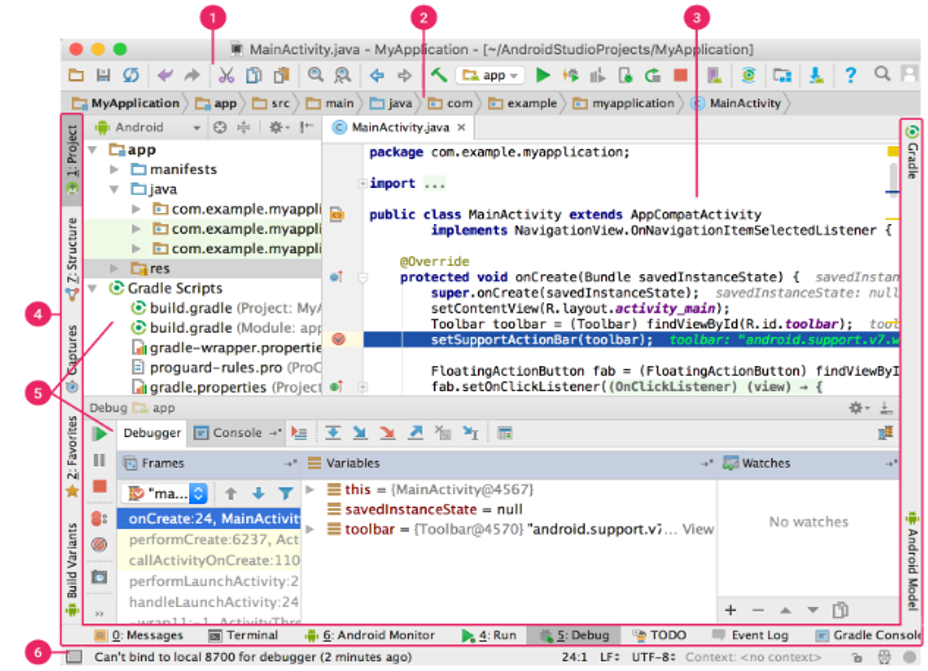
\includegraphics[width=.75\textwidth]{figures/JU.png}
  \caption{Jendela Utama Android Studio}\label{fig:error}
\end{figure}
\begin{enumerate}
\item Toolbar
\hfill \break
Toolbar memungkinkan Anda melakukan berbagai tindakan, termasuk menjalankan aplikasi dan meluncurkan fitur Android
\item Menu Navigasi
\hfill \break
Menu navigasi membnatu Anda menjelajah project dan membuka file untuk di edit. Menu ini memberikan tampilan struktur yang lebih ringkas yang terlihat di jendela Project.
\item Jendela Editor
\hfill \break
Jendela Editor adalah tempat Anda membuat dan memodifikasi kode. Tergantung jenis file yang ada, editor ini dapat berubah. Misalnya, saat menampilkan file tata letak, editor akan menampilkan Layout Editor.
\item Panel Jendela Fitur
\hfill \break
Panel Jendela Fitur berada di sisi luar jendela IDE dan berisi tombol-tombol yang memungkinkan Anda memperluas atau menciutkan setiap jendela fitur.
\item Jendela Fitur
\hfill \break
Jendela Fitur memberi Anda akses ke tugas tertentu seperti pengelolaan project, penelusuran, kontrol versi dan banyak lagi. Anda dapat memperluas dan menciutkan jendela ini.
\item Status Bar
\hfill \break
Status Bar menampilkan status project Anda dan IDE itu sendiri, serta semua peringatan atau pesa.
\end{enumerate}
\section{Bahasa Java}
\hfill \break
Bahasa Pemrograman Java
\begin{figure}[!htbp]
  \centering
  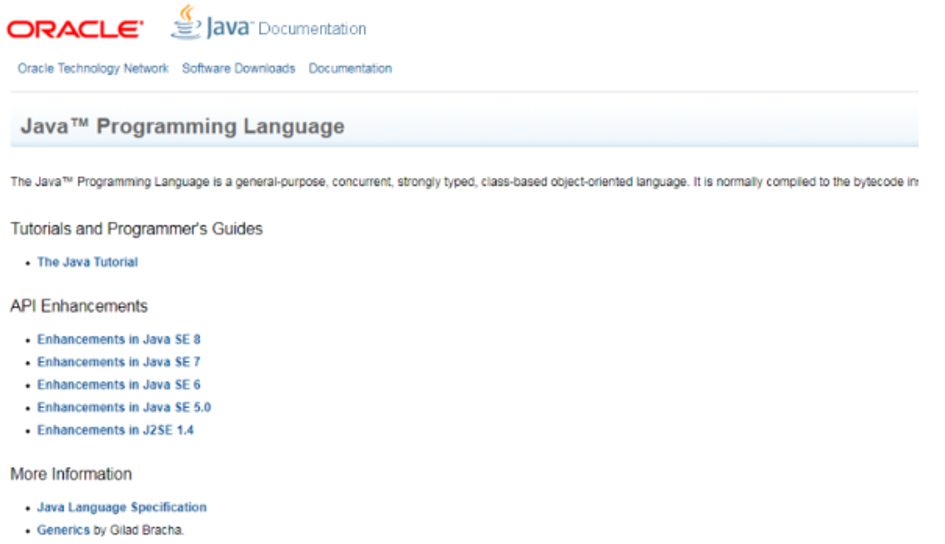
\includegraphics[width=.75\textwidth]{figures/java.png}
  \caption{Bahasa pemrograman yang digunakan untuk menbuat aplikasi ini adalah bahasa Java}\label{fig:error}
\end{figure}
\hfill \break
Bahasa pemrograman java merupakan bahasa yang berada pada urutan 10 besar bahasa pemrograman yang terpopuler di dunia saat ini. Bahasa pemrograman Java pada tahun 2017 merupakan bahasa paling populer, namum sekarang sudah disalip oleh bahasa pemrograman JavaScript dan Python.
\hfill \break
Salah satu penyebabnya yaitu karena jutaan aplikasi android dibuat menggunakan bahasa pemrograman java. Untuk membuat aplikasi android menggunakan bahasa java kita bisa menggunakan tools atau IDE:
\begin{enumerate}
\item Android Studio (IDE resmi didukung penuh oleh google)
\item Eclipse (IDE lain yang sebelumnya didukung penuh oleh google sebelum adanya android studio)
\end{enumerate}
\hfill \break
Untuk pemula yang baru ingin membuat aplikasi android disarankan menggunakan bahasa pemrograman java.
\section{Bahasa Kotlin}
\hfill \break
Bahasa Pemrograman Kotlin
\begin{figure}[!htbp]
  \centering
  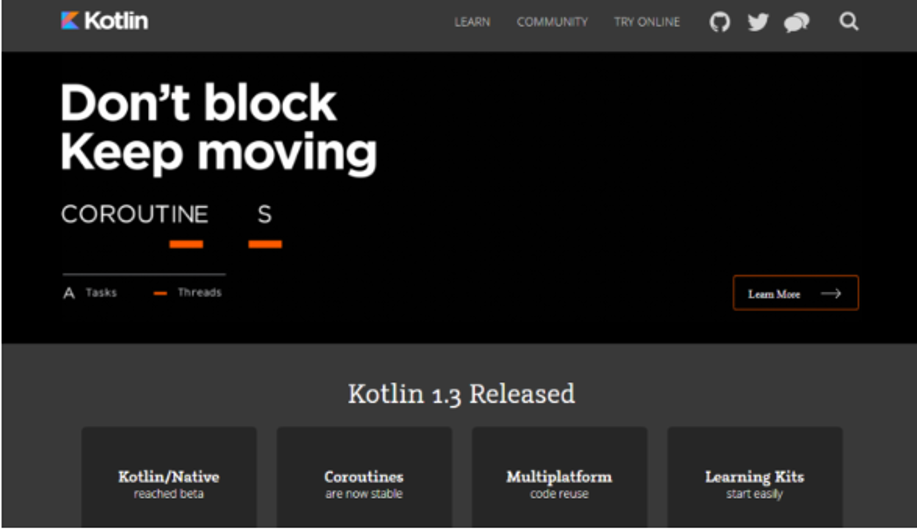
\includegraphics[width=.75\textwidth]{figures/Kotlin.png}
  \caption{Bahasa pemrograman yang digunakan untuk menbuat aplikasi pada android Studio bisa juga menggunakan bahasa kotlin}\label{fig:error}
\end{figure}
\hfill \break
Kotlin dicipyakan oleh JetBrains yaitu perusahaan yang terkenal membuat IDE seperti : Android Studio, RubbyMine,PHPStrome, dll.
\hfill \break
Kotlin sengaja diciptakan oleh JetBrains untuk melengkapi segala kekurangan dari bahasa pemrograman Java. Memang benar bahasa pemrograman kotlin lebih simple dibandingkan Java.
\hfill \break
Keunggulan lainnya dari bahasa Kotlin yaitu bahasa ini bisa berjalan beriringan dengan bahasa pemrograman Java. Dan juga bisa menggunakan library dari Java.
\hfill \break
Pembuatan aplikasi android saat ini bisa menggunakan IDE :
\begin{enumerate}
\item Intellij IDEA
\item Android Studio
\item Eclipse
\end{enumerate}

\chapter{Installasi Android Studio}
\section{Instalasi Android Studio}
Sebelum mengedit alangkah baiknya diinstall terlebih dahulu editornya seperti sebagai berikut :
\begin{enumerate}
	\item Download installernya terlebih dahulu berikut linknya :
\par https://developer.android.com/studio?hl=id.
	\item \textit{Double-click} pada tulisan download android studio pada gambar \ref{fig:installer}
		 \begin{figure}[!htbp]
  		 \centering
 		 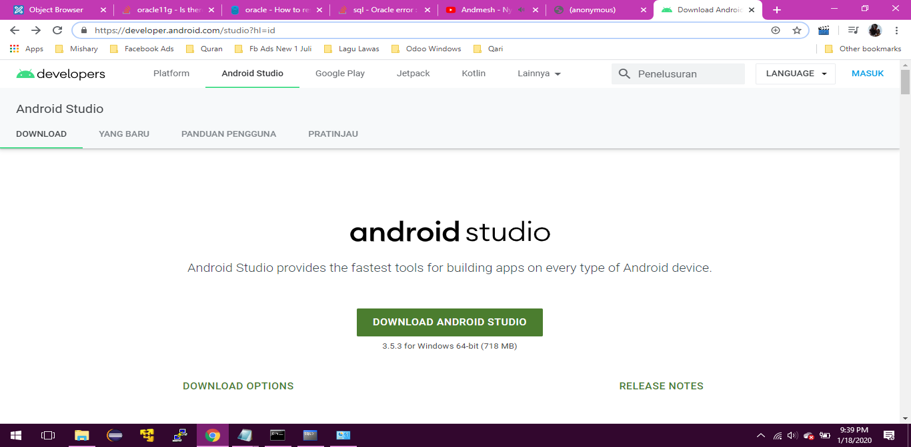
\includegraphics[width=.75\textwidth]{figures/In1.png}
  		 \caption{Ini adalah langkah pertama untuk install Android Studio, buka website resmi Android Studio}\label{fig:installer}
		 \end{figure}
	\item Maka akan muncul halaman awal installer seperti pada gambar  \ref{fig:agreement}
		 \begin{figure}[!htbp]
  		 \centering
 		 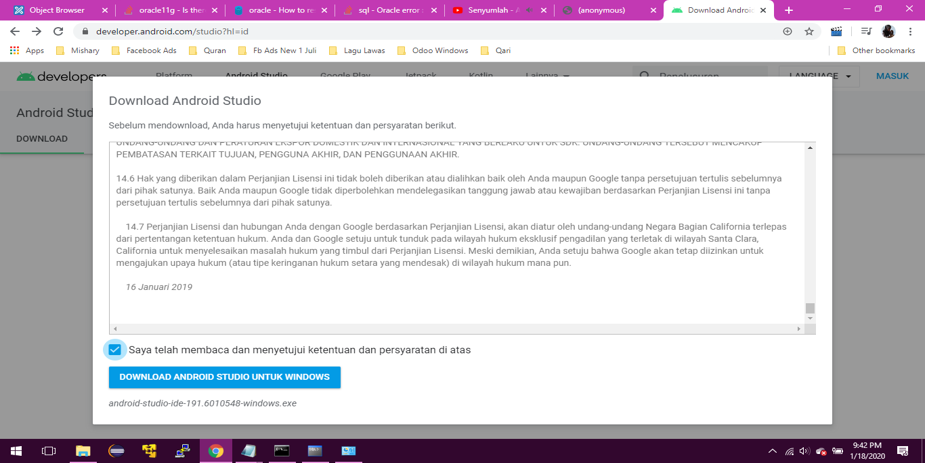
\includegraphics[width=.75\textwidth]{figures/In2.png}
  		 \caption{Ini adalah Halaman persetujuan install}\label{fig:agreement}
		 \end{figure}
	\item Klik \textit{Next} maka akan muncul Halaman installasi scope seperti pada gambar \ref{fig:IS}
		 \begin{figure}[!htbp]
  		 \centering
 		 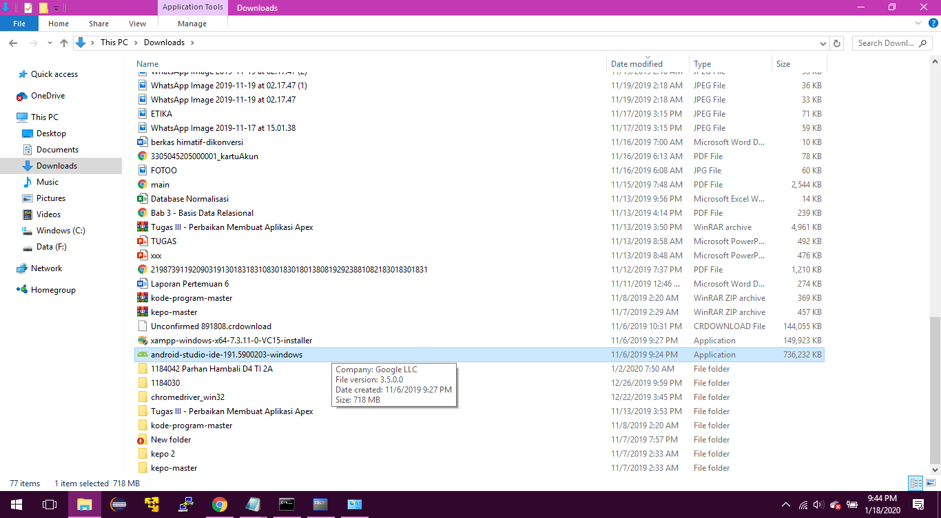
\includegraphics[width=.75\textwidth]{figures/In3.png}
  		 \caption{Ini adalah Halaman istallasi scope}\label{fig:IS}
		 \end{figure}
	\item Klik \textit{Next} maka akan muncul Halaman dari tampilan Android Studio seperti pada gambar \ref{fig:paper}
		 \begin{figure}[!htbp]
  		 \centering
 		 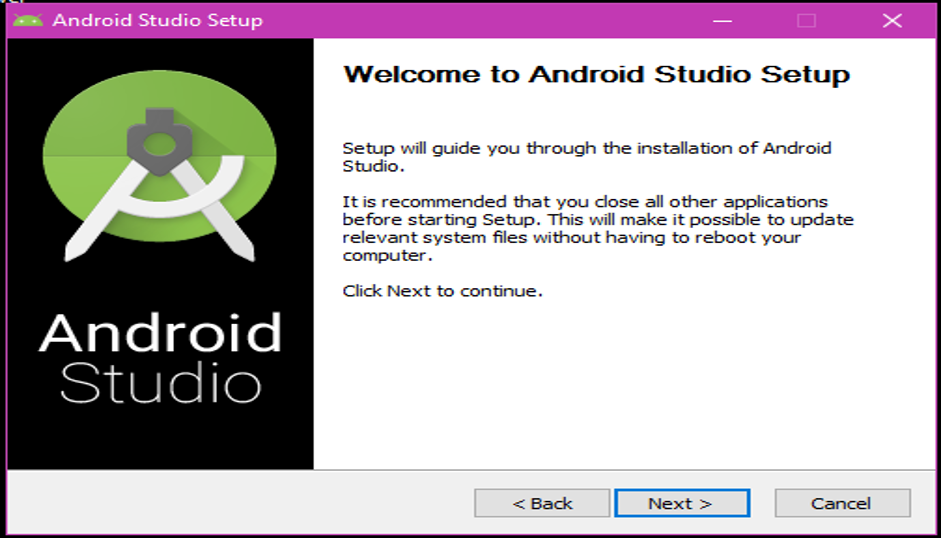
\includegraphics[width=.75\textwidth]{figures/In4.png}
  		 \caption{Ini adalah Halaman penentuan ukuran kertas}\label{fig:paper}
		 \end{figure}
	\item Klik \textit{Next} untuk melanjutkan proses intalasi \ref{fig:dir}
		 \begin{figure}[!htbp]
  		 \centering
 		 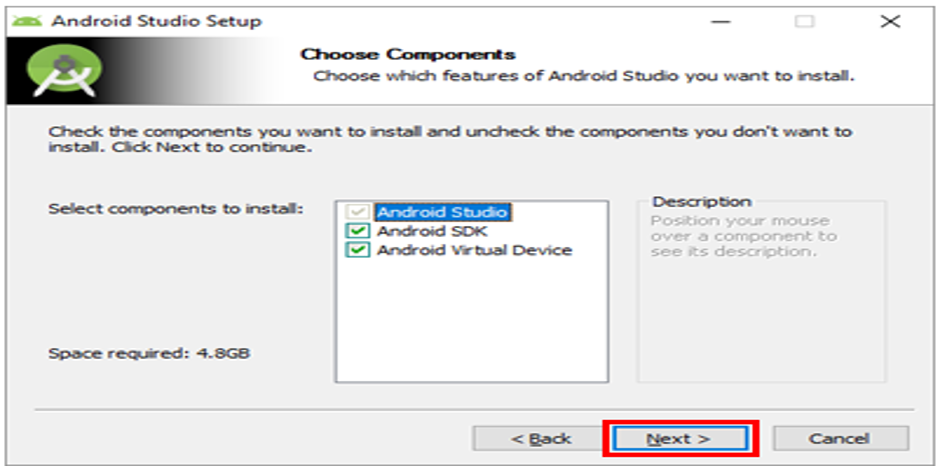
\includegraphics[width=.75\textwidth]{figures/In5.png}
  		 \caption{Ini adalah Halaman Welcome Android Studio}\label{fig:dir}
		 \end{figure}
	\item Klik \textit{Next} maka akan muncul halaman untuk memulai proses install seperti pada gambar \ref{fig:start}
		 \begin{figure}[!htbp]
  		 \centering
 		 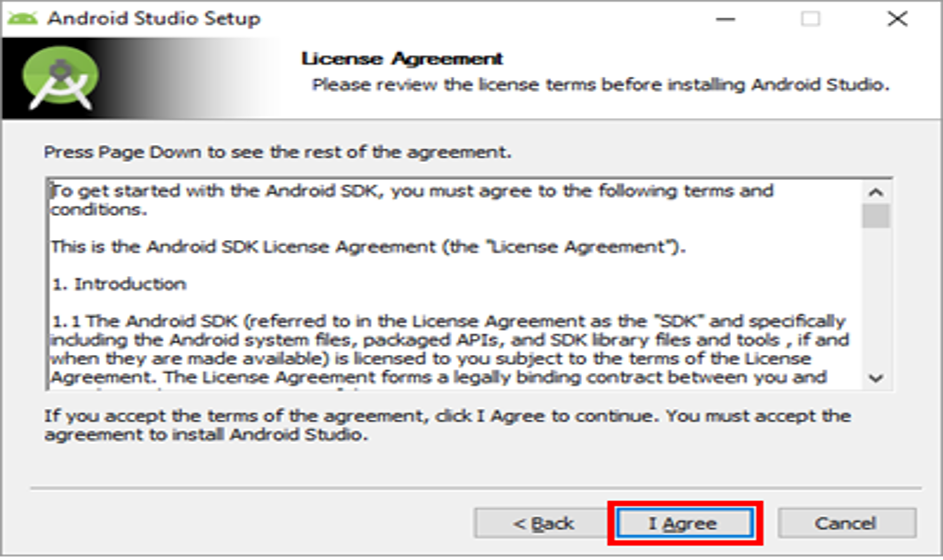
\includegraphics[width=.75\textwidth]{figures/In6.png}
  		 \caption{Ini adalah Halaman memulai install dengan memilih componen Android Studio}\label{fig:start}
		 \end{figure}
	\item Klik \textit{Start} maka proses installasi akan dimulai seperti pada gambar \ref{fig:proses}
		 \begin{figure}[!htbp]
  		 \centering
 		 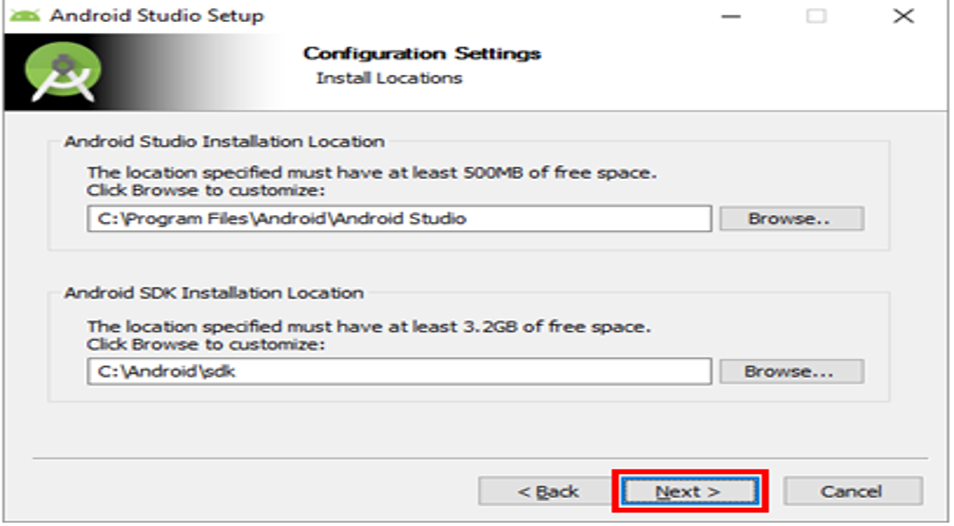
\includegraphics[width=.75\textwidth]{figures/In7.png}
  		 \caption{Ini adalah Proses installasi unutk persetujuan Androis SDK License Agreement}\label{fig:proses}
		 \end{figure}
	\item  Klik \textit{Next} untuk menentukan lokasi penyimpanan Android Studio \ref{fig:ex}
		 \begin{figure}[!htbp]
  		 \centering
 		 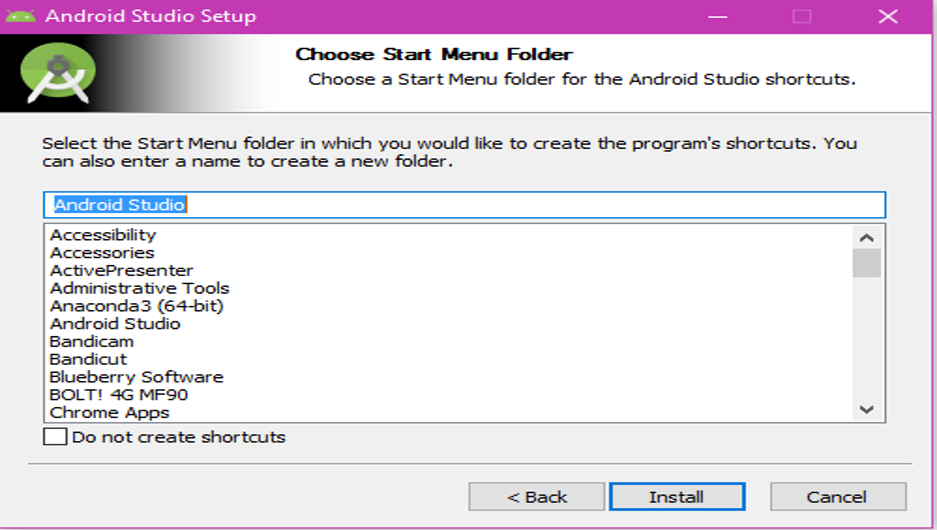
\includegraphics[width=.75\textwidth]{figures/In8.png}
  		 \caption{Ini adalah Halaman untuk penyimpanan Android Studio}\label{fig:ex}
		 \end{figure}
	\item Klik \textit{Install} maka akan muncul halaman seperti pada gambar \ref{fig:done} maka installasi siap untuk dimulai.
		 \begin{figure}[!htbp]
  		 \centering
 		 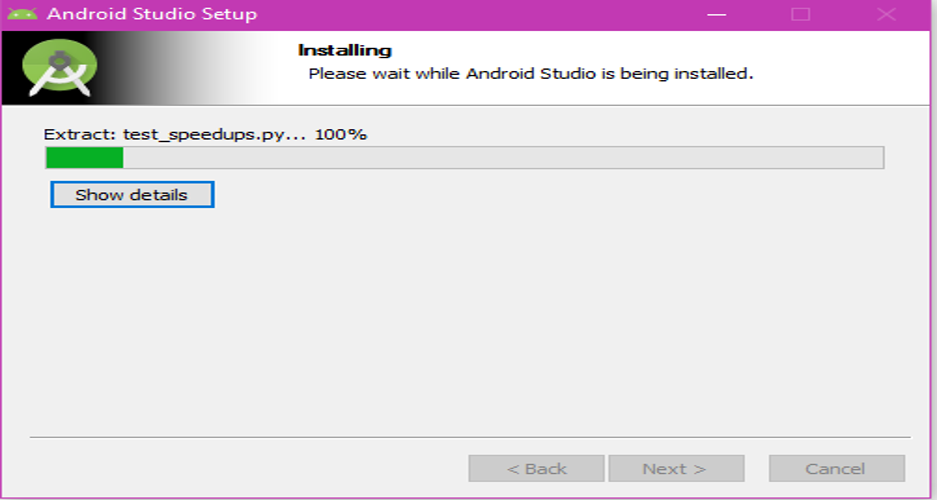
\includegraphics[width=.75\textwidth]{figures/In9.png}
  		 \caption{Installasi segera dimulai}\label{fig:done}
		 \end{figure}
		 \item Klik \textit{Next} maka akan muncul halaman seperti pada gambar \ref{fig:done} maka installasi sedang berjalan, tunggu hingga proses loading berhenti.
		 \begin{figure}[!htbp]
  		 \centering
 		 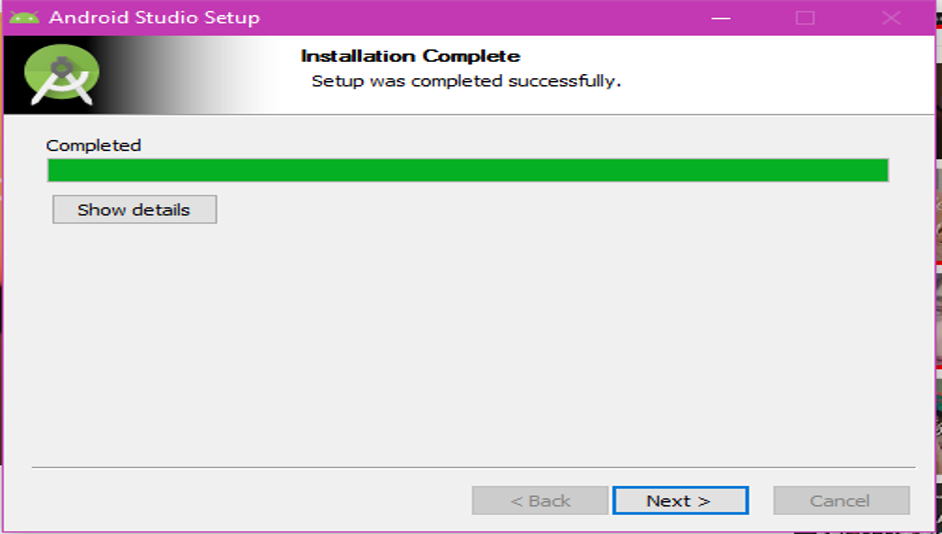
\includegraphics[width=.75\textwidth]{figures/In10.png}
  		 \caption{Installasi sedang berjalan}\label{fig:done}
		 \end{figure}
		 \item Klik \textit{Next} maka akan muncul halaman seperti pada gambar \ref{fig:done} maka installasi siap digunakan.
		 \begin{figure}[!htbp]
  		 \centering
 		 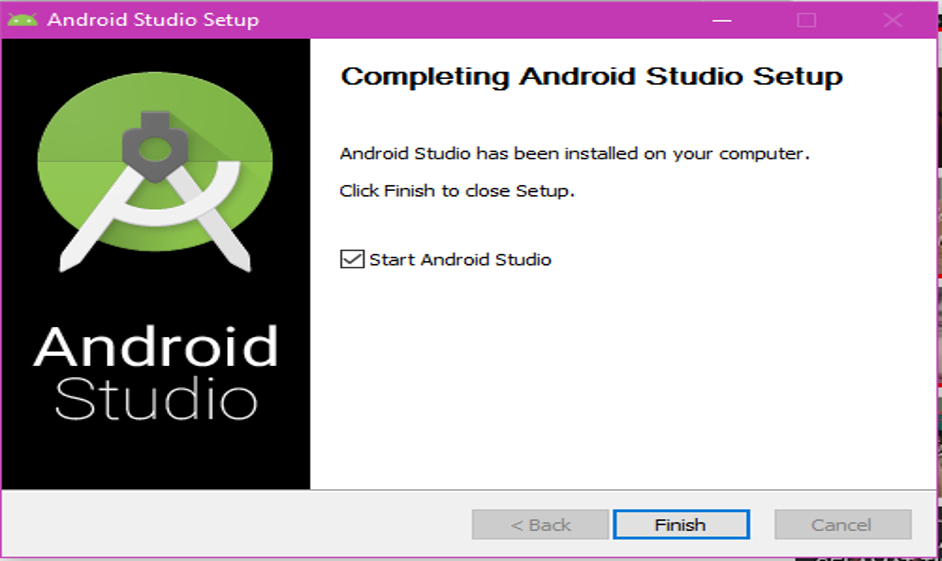
\includegraphics[width=.75\textwidth]{figures/In11.png}
  		 \caption{Installasi sudah selesai}\label{fig:done}
		 \end{figure}
		 \item Klik \textit{Next} maka akan muncul halaman seperti pada gambar \ref{fig:done} maka installasi sudah selesai dilakukan dan program siap digunakan.
		 \begin{figure}[!htbp]
  		 \centering
 		 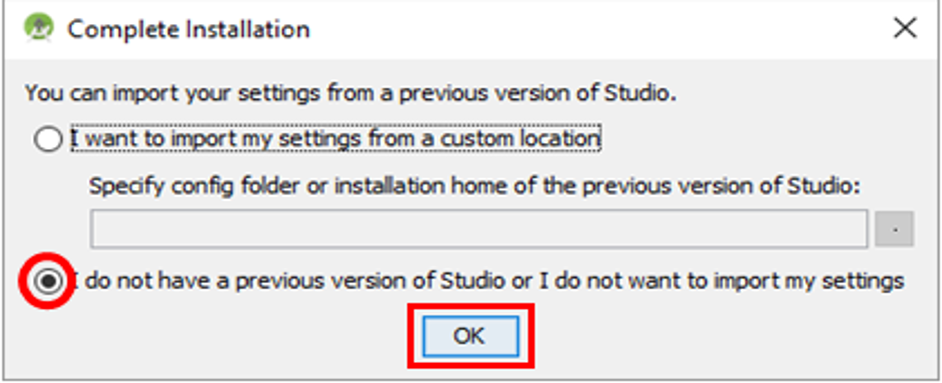
\includegraphics[width=.75\textwidth]{figures/In12.png}
  		 \caption{Installasi sudah selesai}\label{fig:done}
		 \end{figure}
		 \item Klik \textit{Next} maka akan muncul halaman seperti pada gambar \ref{fig:done} disini akan diberikan dua opsi untuk memberikan tanda cheklist pada 2 opsi.
		 \begin{figure}[!htbp]
  		 \centering
 		 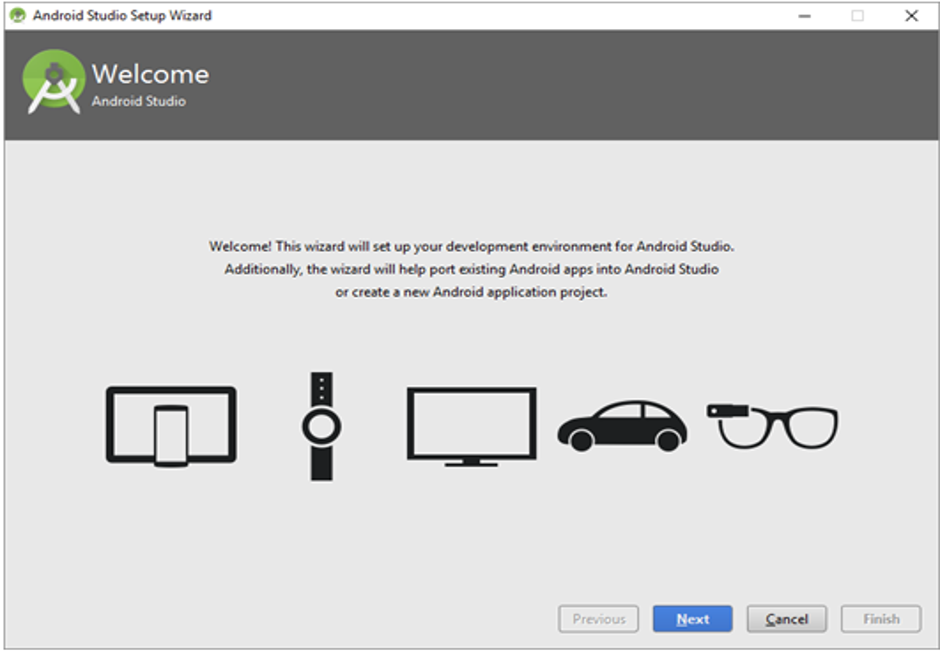
\includegraphics[width=.75\textwidth]{figures/In13.png}
  		 \caption{Pilih untuk yang ada lingkaran merah}\label{fig:done}
		 \end{figure}
		 \item Klik \textit{Next} maka akan muncul halaman seperti pada gambar \ref{fig:done} klik saja next.
		 \begin{figure}[!htbp]
  		 \centering
 		 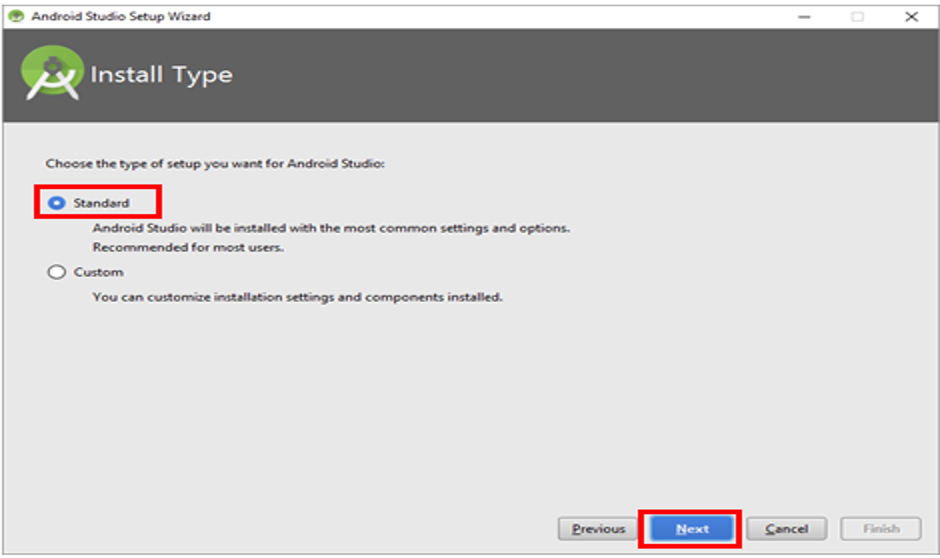
\includegraphics[width=.75\textwidth]{figures/In14.png}
  		 \caption{klik Next}\label{fig:done}
		 \end{figure}
		 \item Klik \textit{Next} maka akan muncul halaman seperti pada gambar \ref{fig:done} maka akan dberikan 2 pilihan tipe untuk Android Studio.
		 \begin{figure}[!htbp]
  		 \centering
 		 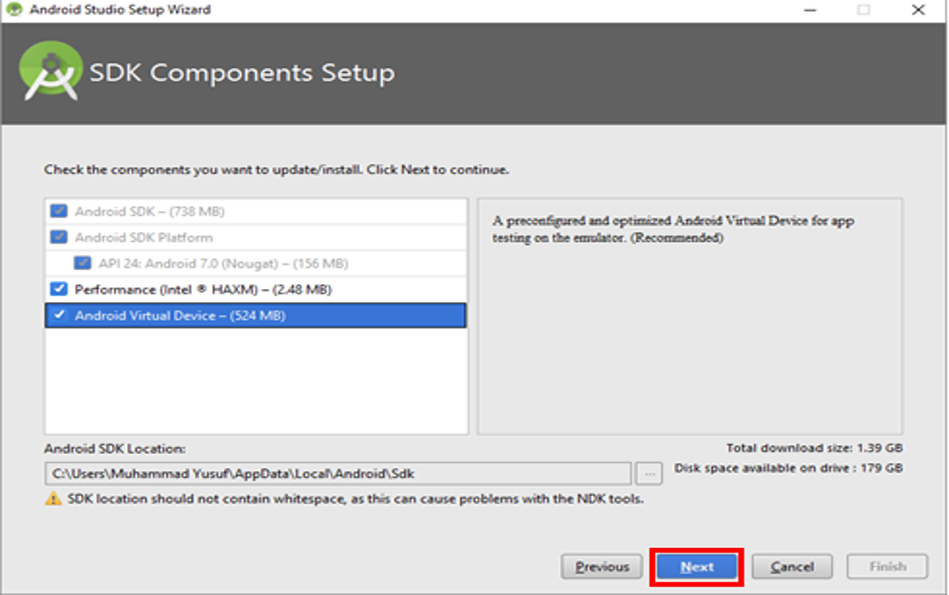
\includegraphics[width=.75\textwidth]{figures/In15.png}
  		 \caption{Pilih yang standard}\label{fig:done}
		 \end{figure}
		 \item Klik \textit{Next} maka akan muncul halaman seperti pada gambar \ref{fig:done} maka pilih yang akan diinstal dan yg dibutuhkan Android Studio
		 \begin{figure}[!htbp]
  		 \centering
 		 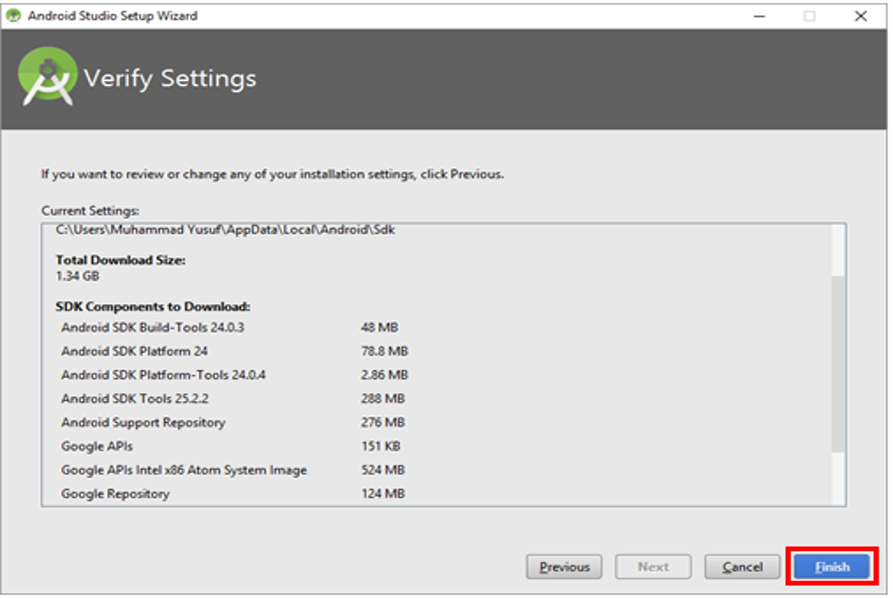
\includegraphics[width=.75\textwidth]{figures/In16.png}
  		 \caption{Pilih sesuai yang ada diatas}\label{fig:done}
		 \end{figure}
		 \item Klik \textit{Next} maka akan muncul halaman seperti pada gambar \ref{fig:done} selanjutnya klik Finsih.
		 \begin{figure}[!htbp]
  		 \centering
 		 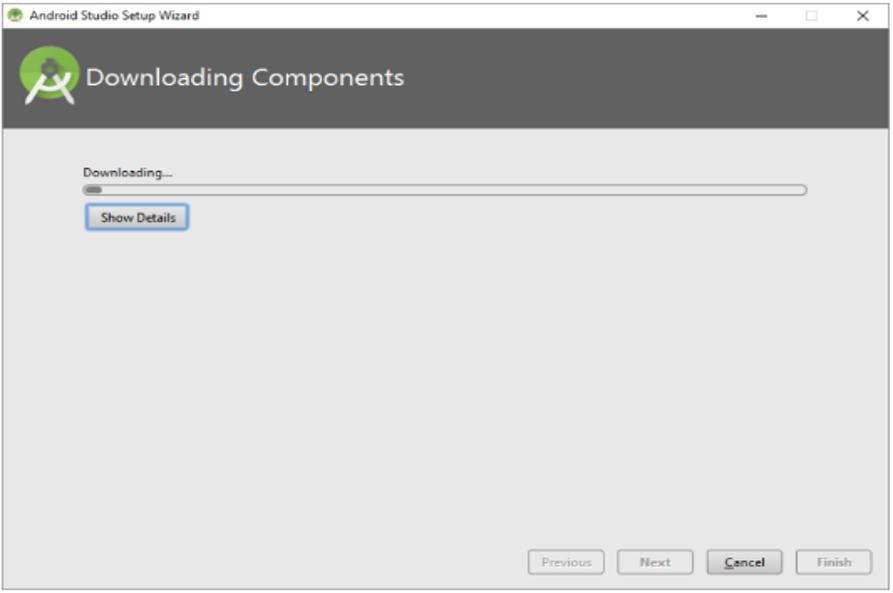
\includegraphics[width=.75\textwidth]{figures/In17.png}
  		 \caption{klik Finsih}\label{fig:done}
		 \end{figure}
		 \item Klik \textit{Next} maka akan muncul halaman seperti pada gambar \ref{fig:done} tunggu hingga proses downloading selesai.
		 \begin{figure}[!htbp]
  		 \centering
 		 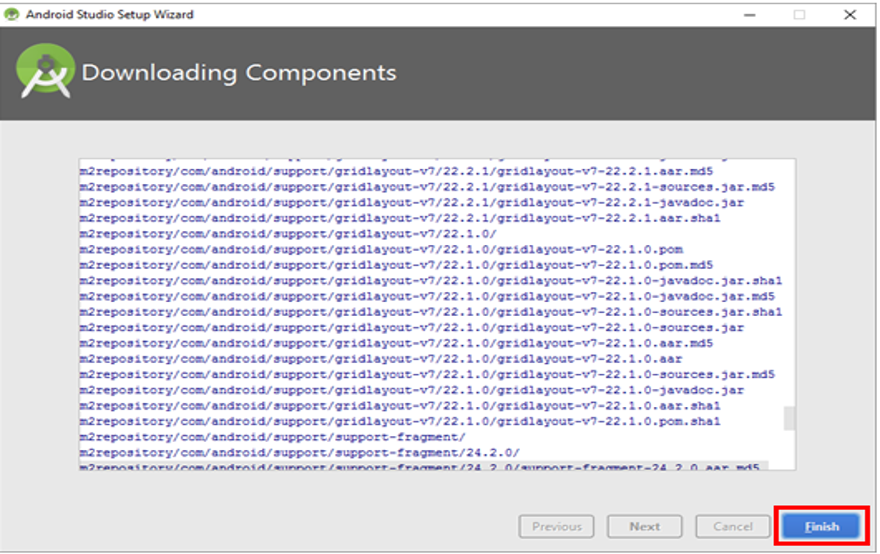
\includegraphics[width=.75\textwidth]{figures/In18.png}
  		 \caption{Tunggu proses downloadng}\label{fig:done}
		 \end{figure}
		 \item Klik \textit{Next} maka akan muncul halaman seperti pada gambar \ref{fig:done} maka installasi sudah selesai dilakukan.
		 \begin{figure}[!htbp]
  		 \centering
 		 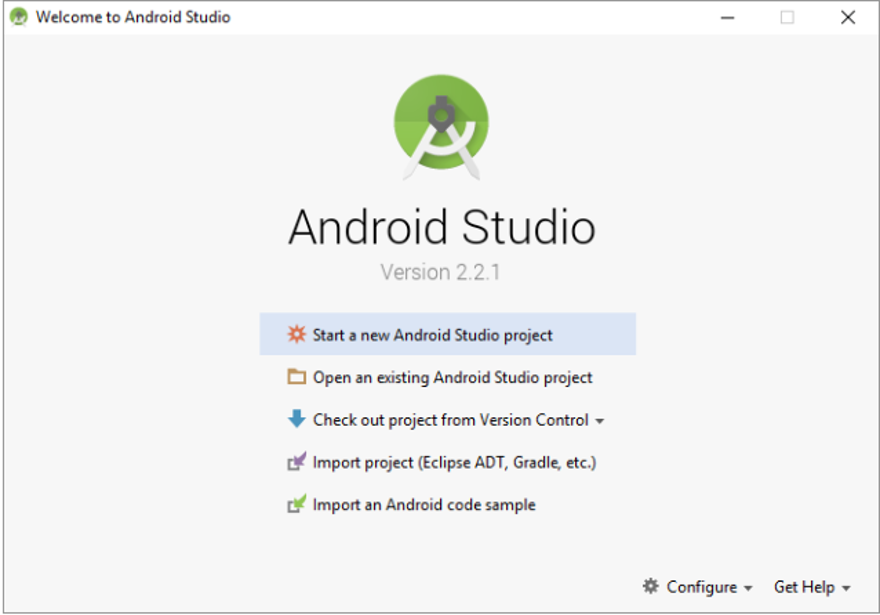
\includegraphics[width=.75\textwidth]{figures/In19.png}
  		 \caption{Installasi sudah selesai}\label{fig:done}
		 \end{figure}
		 \item Klik \textit{Next} maka akan muncul halaman seperti pada gambar \ref{fig:done} maka installasi sudah siap digunakan.
		 \begin{figure}[!htbp]
  		 \centering
 		 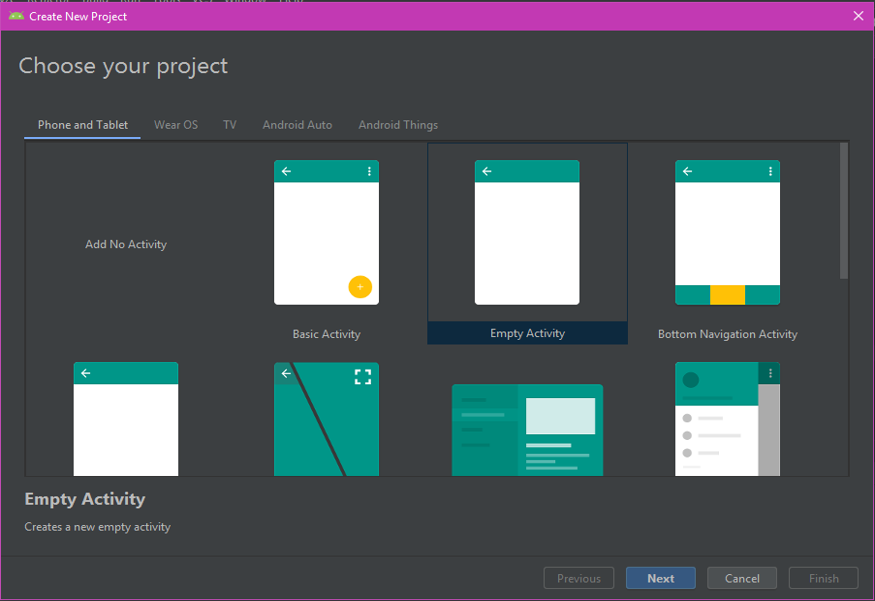
\includegraphics[width=.75\textwidth]{figures/In20.png}
  		 \caption{Andrid Studio siap digunakan}\label{fig:done}
		 \end{figure}
\end{enumerate}


\chapter{Pengenalan PHP}
\section{Sejarah PHP}
\subsection{PHP/FI : Personal Home Page/Forms Interpreter}
Sejarah PHP bermula pada tahun 1994 keika programmer kelahiran Denmark yang sekarang berdomisili di Canada, Rasmus Lerdorf membuat sebuah script(Kode Program) dengan bahasa Perl unutk web pribadinya. Salah satu kegunaan script ini adalah untuk menampilkan resume pribadi dan mencatat jumlah pengunjung ke sebuah website.
\hfill \break
Dengan alasan untuk meningkatkan performa, Rasmus Lerdorf kemudian membuat ulang kode program tersebut dadlam bahasa C. Ia juga mengembangkannya lebih lanjut sehngga memiliki script tersebut dan memiliki kemampuan unutk memproses form HTML dan berkomunikasi dengan database.
\hfill \break
Lerdorf menyebut kode program ini sebagai Personal Home Pages/Form Interpreter atau PHP/FI. Inilah asal mula penanaman PHP digunakan. PHP/FI dapat digunakan untuk membuat aplikasi web dinamis sederhana.
\hfill \break
Lerdorf kemudian merilis kode tersebut ke publik dengan sebutan Personal Home Page Tools9PHP Tools)version 1.0. 
\subsection{PHP/FI : Personal Home Page/Forms Interpreter 2}
\hfill \break
Seiring dengan pengembangan dan penambahan fitur web pada saat itu, April 1996, Rasmus Lerdrof mengumumkan PHP/FI Versi 2.0. PHP versi 1 sebenernya sudah mencukupi, namun performa yang dihasilkan dirasakan belum cukup, sehingga butuh penambahan fitur lanjutan.
\subsection{PHP:Hypertext Preprocessor 3}
\hfill \break
Evolusi PHP berikutnya terjadi pada pertengahan tahun 1997, PHP versi 2 telah menarik banyak perhatian programmer, namun bahasa ini memiliki masalah dengan kestabilan yang kurang bisa diandalkan. Hal ini di karenakan Lerdorf hanya bekerja sendiri untuk mengembangkan PHP.
\hfill \break
Dengan dukungan banyak programmer lainnnya, Proyek PHP secara perlahan beralih dari proyek satu orang menjadi proyek massal yang lebih di akrab kita kenal sebagai open-source project. PHP selanjutnya dikembangkan oleh The PHP Group yang merupakan kumpulan banyak programmer dari seluruh dunia.
\hfill \break
Perilisan PHP Versi 3 juga ditandai dengan perubahab singkatan PHP yang sebelumnya PHP/FI:Personal Home Pages Tools, menjadi PHP : Hypertext Preprocessor. Kepanjangan PHP sebagai PHP:Hypertext Preprocessor disebut juga sebagai kepanjangan rekursrif, sebuah istilah dalam pemrograman diaman suatu fungsi memanggil dirinya sendiri.
\hfill \break
Setelah perilisan PHP 3.0, PHP semakin populer digunakan di seluruh dunia. Dan sejak saat itu, penggunaan PHP sebagai bahasa pemrograman web menjadi sebuah standar bagi programmer.
\subsection{PHP:Hypertext Preprocessor 4}
\hfill \break
Segera setelah, Zeev Suraski,Andi Gutmans dan juga brbagai programmer di seluruh dunia mengembangkan PHP lebih jauh lagi dengan memperkenalkan banyak fitur lanjutan, seperti layer abstraksi antara PHP dengan web server, menambahkan mekanisme thread-safety dan two-stage parsing. Parsing baru ini dikemabangkan oleh Zeev dan Andi dan dinamakan Zend engine. Akhirnya pada 22 May 2000 diluncurkan PHP 4.0
\hfill \break
PHP versi 4 jga menyertakan fitur pemrograman objek/{object Oriented Programming, walaupun belum sempurna.
\subsection{PHP:Hypertext Preprocessor 5}
\hfill \break
Versi PHP terakhir hingga saat ini, yaitu PHP 5.x diluncurkan pada 13 juli 2004. PHP 5 telah mendukung penuh pemrograman object dan peningkatan performa melalui Zend engine versi 2.
\hfill \break
Beberapa penambahan fitur meliputi PDO(PHP Data Object) untuk pengaksesan database, closures, tarit dan namespaces.
\subsection{PHP:Hypertext Preprocessor 6}
\hfill \break
Versi lanjutan dari PHP , yakni PHP 6.x sebenernya telah lama dikembangkan, bahkan sejak tahu 2005. Fokus pengembangan PHP 6 terutama dalam mendukung Unicode agar PHP bisa mendukung berbagai jenis karakter bahasa non-latin.
\hfill \break
Namun karena beberapa alasan seperti kurangnya programmer dan performa yang tidak memuaskan, pengembangan PHP 6 dihentikan dan fitur yang ada dimasukkan ke dalam PHP 5. 
\subsection{PHP:Hypertext Preprocessor 7}
\hfill \break
Pada tanggal 3 Desember 2015, PHP 7 resmi dirilis. Perubahan yang paling terlihat adalah peningkatan performa. Menggunakan Zend Engine 3, PHP 7 di klaim berjalan 2 kali lebih cepat daripada PHP 5.6. Proyek ini menggunakan pendekatan modern agar PHP diproses dengan lebih cepat seperti memakai teknik just-in-time(JIT) compiler.
\hfill \break
Walaupun terkendala dengan perilisan PHP versi 6. PHP 7 saat ini menjadi versi PHP terbaru dan versi yang disarankan.


\chapter{Webhost000}
\section{Pengertian Web Hosting}
\hfill \break
Web Hosting adalah sebuah komputer yang terhubung ke internet dan dipergunakan untuk menyimpan data website agar dapat diakses secara online. 
\hfill \break
Dengan memakai web hosting ini maka seluruh informasi yang disimpan dapat ditampilkan.Semua informasi yang disimpan di sebuat tempat disebut server web hosting. Untuk bisa tersabung ke internet dan dapat diakses oleh semua orang, server web hosting dikelola dalam ruang penyimpanan data bernama daat center.
\hfill \break
Istiah web hosting sendiri merujuk pada set aktivitas atau layanan penyimpanan informasi sautu website hingga akhirnya bisa ditampilkan ketika Anda akses. 

\section{Cara Kerja Web Hosting}
\hfill \break
\begin{figure}[!htbp]
  		 \centering
 		 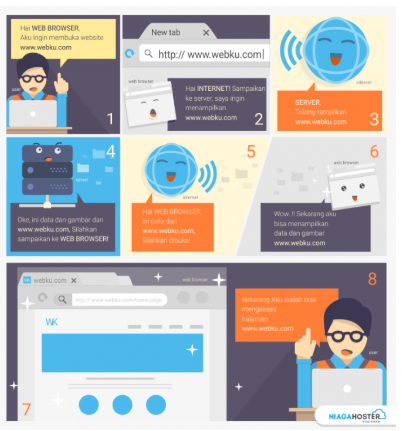
\includegraphics[width=.75\textwidth]{figures/web.png}
  		 \caption{Cara Kera web hosting}\label{fig:done}
		 \end{figure}
\hfill \break
Ketika teman-teman ingin mengases suatu website, maka teman-teman perku mengetikkan alamat website pada browser yang teman-teman gunakan.
\hfill \break
Kemudian, browser akan mengeksekusi perintah yang akan diteruskan dari internet ke server hosting sesuai permintaan. Hasil nya yaitu akan menampilkan gambar dan informasi website sesuai yang di akses dan akan diteruskan oleh internet agar tampil pada browser teman-teman. Jadi, begitulah cara kerja web hosting.



\chapter{Database}
\section{Pengertian Database}
\hfill \break
Database atau basis data adalah kumpulan berbagai data dan informasi yang tersimpan dan tersusun di dalam komputer secara sistematik yang dapat diperiksa, diolah atau dimanipulasi dengan menggunkan program komputer untuk mendapatkan informasi dari basis data tersebut. 
\hfill \break\
Istilah database sendiri mengacu pada koleksi data-data yang saling terkait satu sama lain dimana tujuan database dapat digunakan untuk mengelola data dengan lebih efektif dan efisien. 
\section{Fungsi Database}
\hfill \break\
Setelah memahami apa itu database, maka kita harus mengetahui apa itu fungsi database:
\begin{enumerate}
\item Mengelompokkan data dan informasi sehingga lebih mudah dimengerti
\item Mencegah terjadinya duplikat data maupun inkonsistensi data
\item Mempermudah proses penyimpanan,akses,pembaharuan, dan menghapus data.
\item Menjaga kualitas data dan informasi yang diakses sesuai dengan yang di-input.
\item Membantu proses penyimpanan data yang besar.
\item Membantu meningkatkan kinerja aplikasi yang membutuhkan penyimpanan data.
\end{enumerate}
\section{Manfaat Database}
Berikut beberapa manfaat dari menggunakan database yang bisa didapatkan jika bekerja dengan sistem database:
\begin{enumerate}
\item Tidak terjadinya redudansi Basis Data
\hfill \break
Database mampu meminimalkan terjadinya redudansi artinya redudansi sendiri itu merupakan terjadinya data-data ganda dalam berkas-berkas yang berbeda. 
\item Integritas Data Terjaga
\hfill \break
Database memastikan integritas data yang tinggi dimana database akan memastikan keakuratan,aksesbilitas, konsistensi dan juga kualitas tinggi pada suatu data.
\item Independensi Berbagai Data
\hfill \break
Database menjaga independensi data dimana orang lain tidak dapat merubah data meskipun data bisa diakses.
\item Kemudahan berbagai Data
\hfill \break
Menggunkan perangkat lunak database bisa digunakan untuk berbagi data atau informasi dengan sesa pengguna lainnya.
\item Menjaga Keamanan Data
Database menjamin keamanan suatu informasi data, dimana anda bisa meyisipkan kode akses untuk data-data tertentu yang tidak bisa diakses bersama.
\item Kemudahan Akses Data
\hfill \break
Dengan database bisa memudahkan untuk mengakses dan mendapatkan data karena semua data terorganisir dengan baik.
\end{enumerate}

\section{Maria DB}
\hfill \break
Disini kita akan mencoba untuk membahas berbagai macam tutorial mengenai Maria DB seperti cara install database MariaDB,Syntax,Tipe Data,koneksi,database,membuat database,memilih databsae,membuat tabel,operasi CRUD,cara insert,cara limit,cara update,cara delete,statement dan berbagai perintah bisa digunakan dalam MariaDB.
\hfill \break
Nah, sebelum masuk untuk mempelajari MariaDB ada baiknya jika teman-teman sudah mempelajari atau mengetahui dasar-dasar perintah MYSQL.
\hfill \break
MariaDB adalah proyek berbasis komunitas dari sistem manajemen basis data relasional MYSQL. MariaDB adalah teknologi database open source dan relasional yang dapat digunakan sebagai pengganti MYSQL.Maria DB dikembangkan oleh pengembang asli MYSQL yang khawatir setelah MYSQL diakuisisi oleh Oracle.
\hfill \break
Maria DB adalah relasional database manajemen sistem yang meyimpan data kedalam tabel-tabel yang ada didalam database.Primary Key dan Foreign Key digunakan untuk membangun relasi antar beberapa tabel yang berbeda.
\hfill \break
Relasional databsae manajemen sistem (RDBMS) memiliki beberapa fitur seperti berikut ini:
\begin{enumerate}
\item RDBMS memfasilitasi Anda untuk menerapkan sumber data dengan tabel, kolom, dan indeks.
\item RDBMS menyediakan integritas referensi antar baris dari beberapa tabel.
\item Hal ini digunakan untuk secara otomatis untuk memperbarui indeks.
\item RDBMS dapat diguanakan untuk menafsirkan query SQL dan operasi dalam memanipulasi atau sumber data dari tabel.
\end{enumerate}
\section{Istilah yang digunakan dalam RDBMS}
\hfill \break
Berikut ini adalah beberapa istilah yang digunakan dalam relasional database manajemen sistem pada MariaDB:
\begin{enumerate}
\item Datbase : Database merupakan suatu wadah yang berisi tabel-tabel yang berisi data
\item Table : Tabel merupakan struktur matrix yang berisi data.
\item Coloumn : Coloumn(kolom) adalah suatu elemen data. Coloumn merupakan suatu struktur yang menyimpan data dengan tipe yang sama.
\item Row : Row atau abris adalah struktur dimana suatu data disimpan, Row biasa disebut juga dengan tuple, entry atau record.
\item Primary Key : Primary Key merupakan suatu nilai yang unik. Nilai yang berupa Primary Key tidak dapat muncul dua kali didalam tabel yang sama.
\item Foreign Key : Foreign Key biasanya digunakan untuk menghubungkan dua buah tabel yang berbeda.
\end{enumerate}



\chapter{Flowmap}
\section{Membuat Penomoran Referensi}
Untuk menambahkan referensi atau melakukan sanitasi pada latex kita dapat menggunakan berbagai macam cara. Salah satu cara sederhana yang dapat kita gunakan adalah dengan menggunakan environment yang di sebut \textit{thebibliography}. Namun, kebanyakan orang saat ini menggunakan \textit{BibTeX} untuk melakukan sanitasi sebagai acuan referensi. Dengan menggunakan \textit{BibTex} kita dapat mengatur sitasi sendiri secara terpisah dalam format file \*.bib \cite{atmaja2015tutorial}. Disaat mengutip maupun menggunakan sanitasi diperkenankan untuk memberi keterangan referensi atau sumber asal suatu kutipan dan gagasan. Untuk mengetahui bagaimana menambahkan referensi pada latex, kita dapat melihat langkah-langkahnya seperti pada gambar \ref{fig:contohpenomoranref}.
\begin{figure}[!htbp]
  \centering
  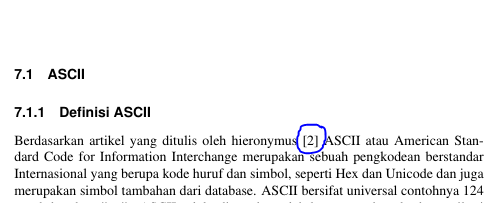
\includegraphics[width=.75\textwidth]{figures/contohpenomoranref.png}
  \caption{Ini adalah Contoh Penomoran Referensi}\label{fig:contohpenomoranref}
\end{figure}
\par Bagaimana cara membuatnya di Latex? berikut cara membuatnya:
\begin{enumerate}
  \item Cari materi yang akan dikutip melalui Google Scholar seperti pada gambar \ref{fig:scholar} ,
  \begin{figure}[!htbp]
  \centering
  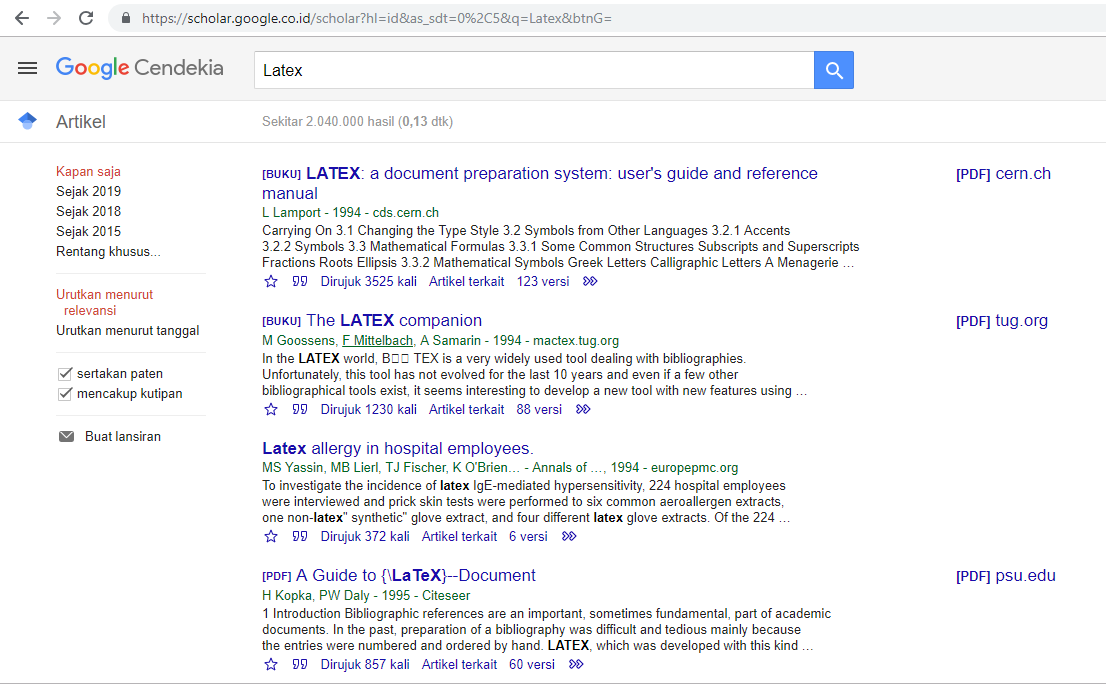
\includegraphics[width=.75\textwidth]{figures/scholar.png}
  \caption{Ini adalah Halaman Google Scholar}\label{fig:scholar}
\end{figure}
  \item Setelah selesai mengutip jangan lupa untuk mengambil script bibtexnya dengan cara klik pada tanda kutip seperti pada gambar \ref{fig:awalbibtex},
  \begin{figure}[!htbp]
  \centering
  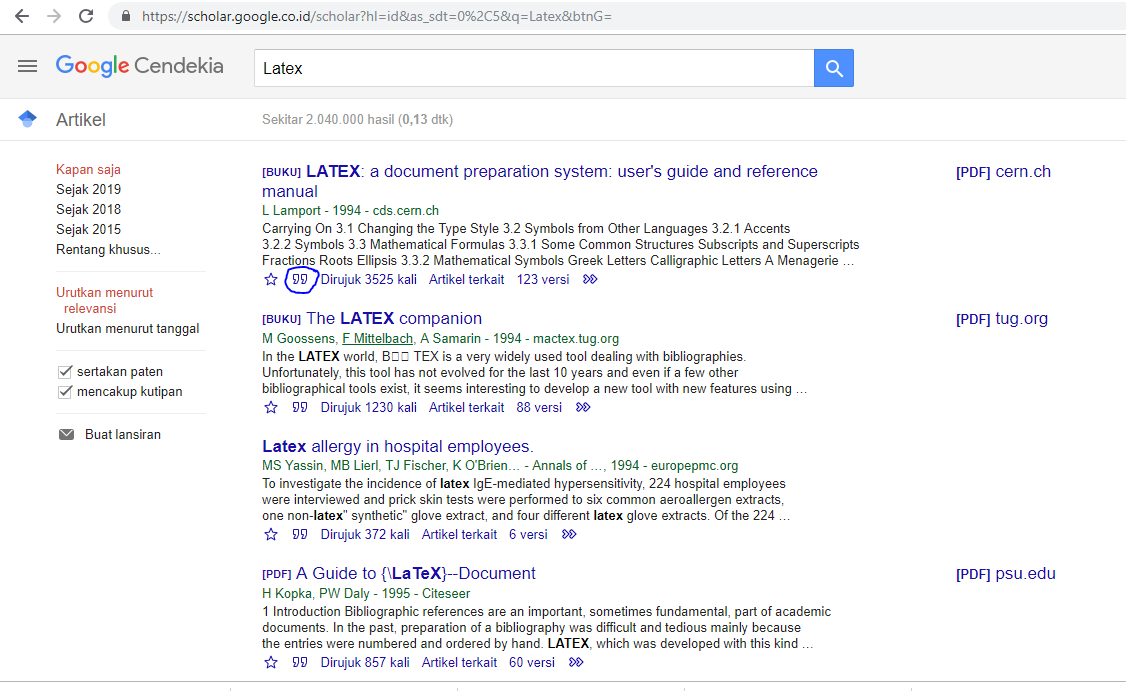
\includegraphics[width=.75\textwidth]{figures/awalbibtex.png}
  \caption{Ini adalah Tanda proses awal mengambil reference}\label{fig:awalbibtex}
\end{figure}
  \item Maka akan muncul seperti gambar \ref{fig:kutip}, lalu pilih Bibtex.
  \begin{figure}[!htbp]
  \centering
  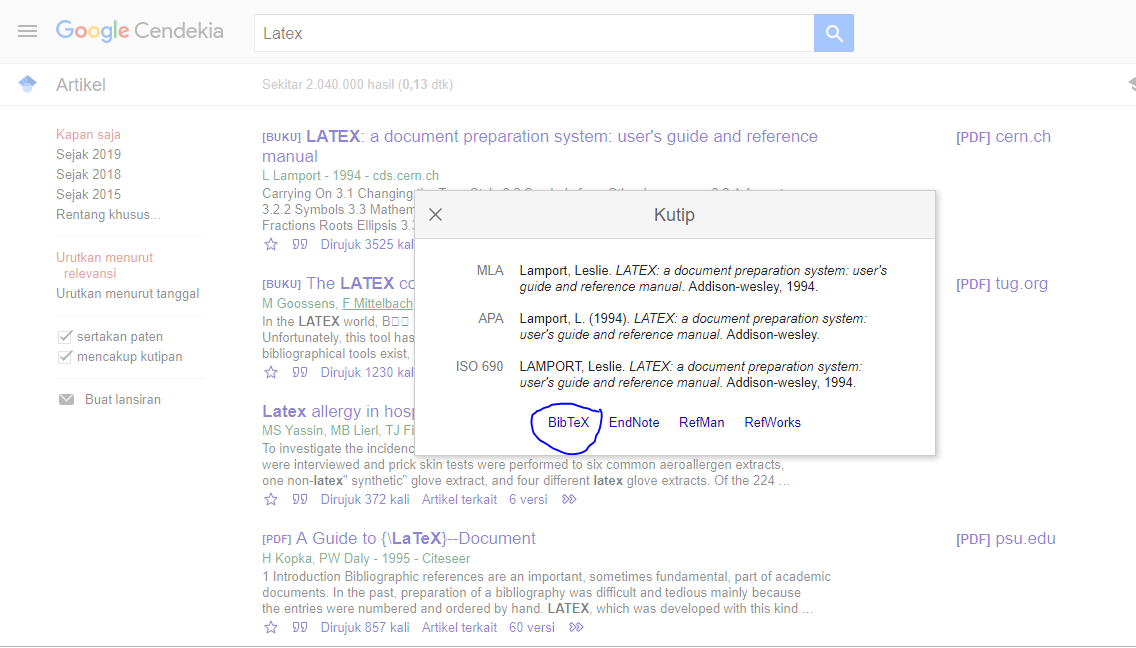
\includegraphics[width=.75\textwidth]{figures/kutip.png}
  \caption{Ini adalah Pilihan mengutip}\label{fig:kutip}
\end{figure}
  \item Setelah memilih Bibtex maka akan muncul script seperti pada gambar \ref{fig:scriptbibtex},
  \begin{figure}[!htbp]
  \centering
  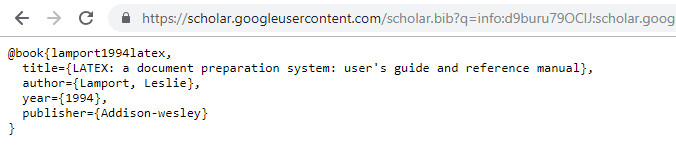
\includegraphics[width=.75\textwidth]{figures/scriptbibtex.png}
  \caption{Ini adalah Script BibTex}\label{fig:scriptbibtex}
\end{figure}
  \item Script tersebut dicopy pada direktori yang dikerjakan, khususnya pada bagian reference.bib seperti pada gambar \ref{fig:direktori} dan \ref{fig:reference} pada editor,
  \begin{figure}[!htbp]
  \centering
  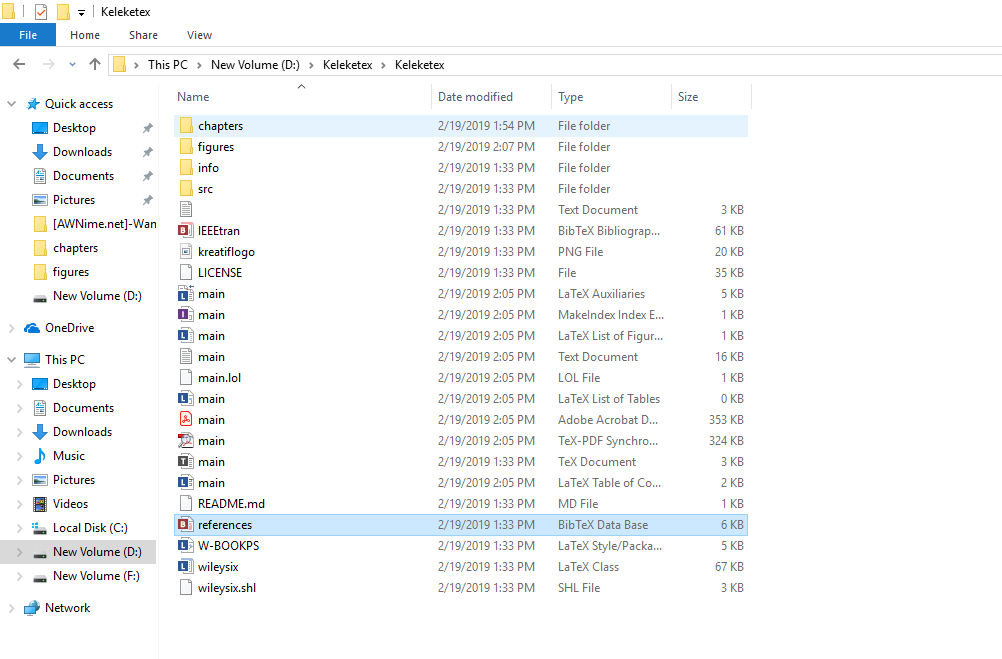
\includegraphics[width=.75\textwidth]{figures/direktori.png}
  \caption{Ini adalah Direktori pekerjaan}\label{fig:direktori}
\end{figure}
\begin{figure}[!htbp]
  \centering
  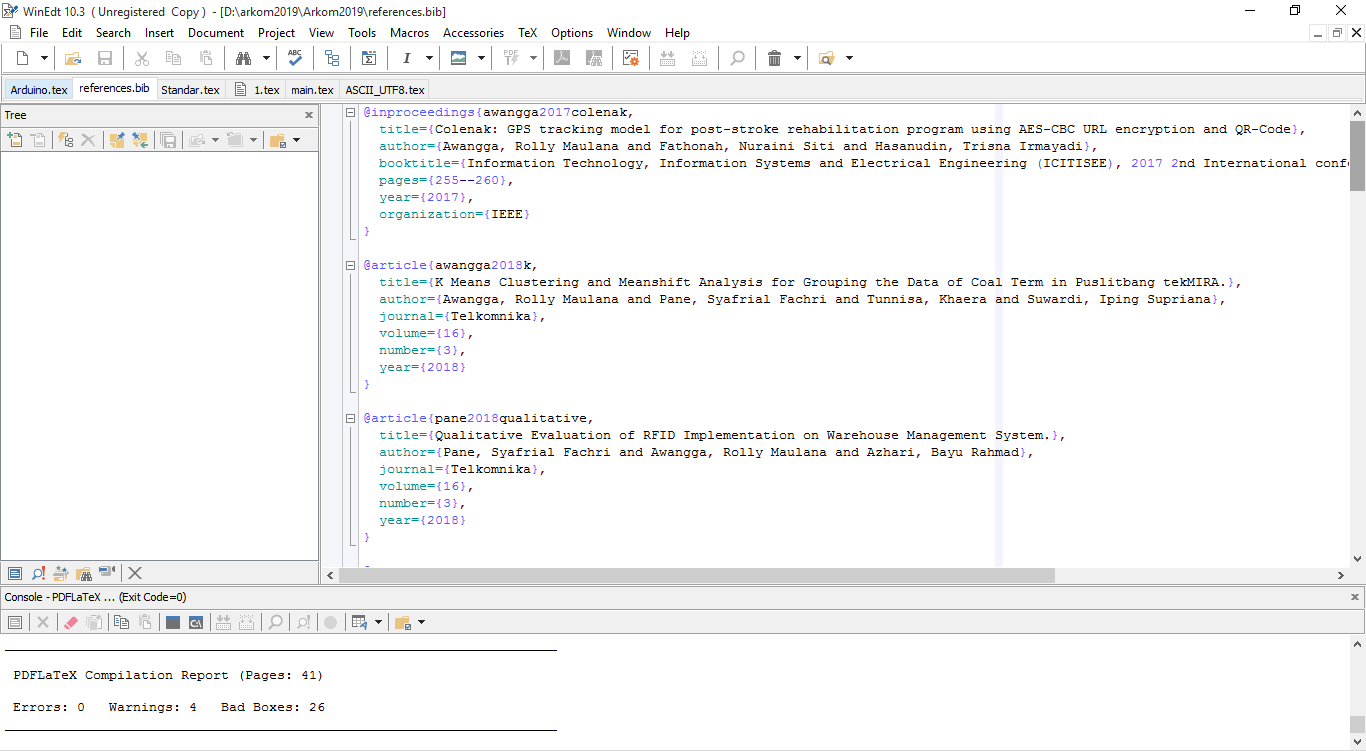
\includegraphics[width=.75\textwidth]{figures/reference.png}
  \caption{Ini adalah Reference.bib}\label{fig:reference}
\end{figure}
  \item Setelah dicopy, jangan lupa disave.
  \item Buka kembali pada lembar kerja yang sudah diberi kutipan/gagasan. Lalu tambahkan script listing \ref{lst:capaian}. setelah kutipan maka akan muncul seperti pada gambar \ref{fig:memilihsumber},
\lstinputlisting[caption=Penggunaan perintah cite untuk reference,label={lst:capaian}]{src/1/reference.tex}
  \begin{figure}[!htbp]
  \centering
  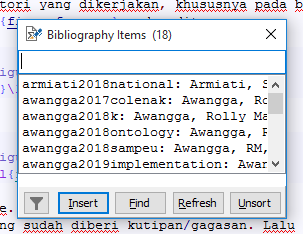
\includegraphics[width=.75\textwidth]{figures/memilihsumber.png}
  \caption{Ini adalah Proses pemilihan sumber}\label{fig:memilihsumber}
\end{figure}
  \item Pilih insert dan save.
  \item Untuk proses compilenya dilakukan 2 kali yaitu pada main.tex pilih Tex lalu pilih pdflatex dan Bibtex, dilakukan berulang minimal 3 kali compile. Seperti pada gambar \ref{fig:pdflatex} untuk pdflatex dan \ref{fig:bibtexx} untuk BibTex.
   \begin{figure}[!htbp]
  \centering
  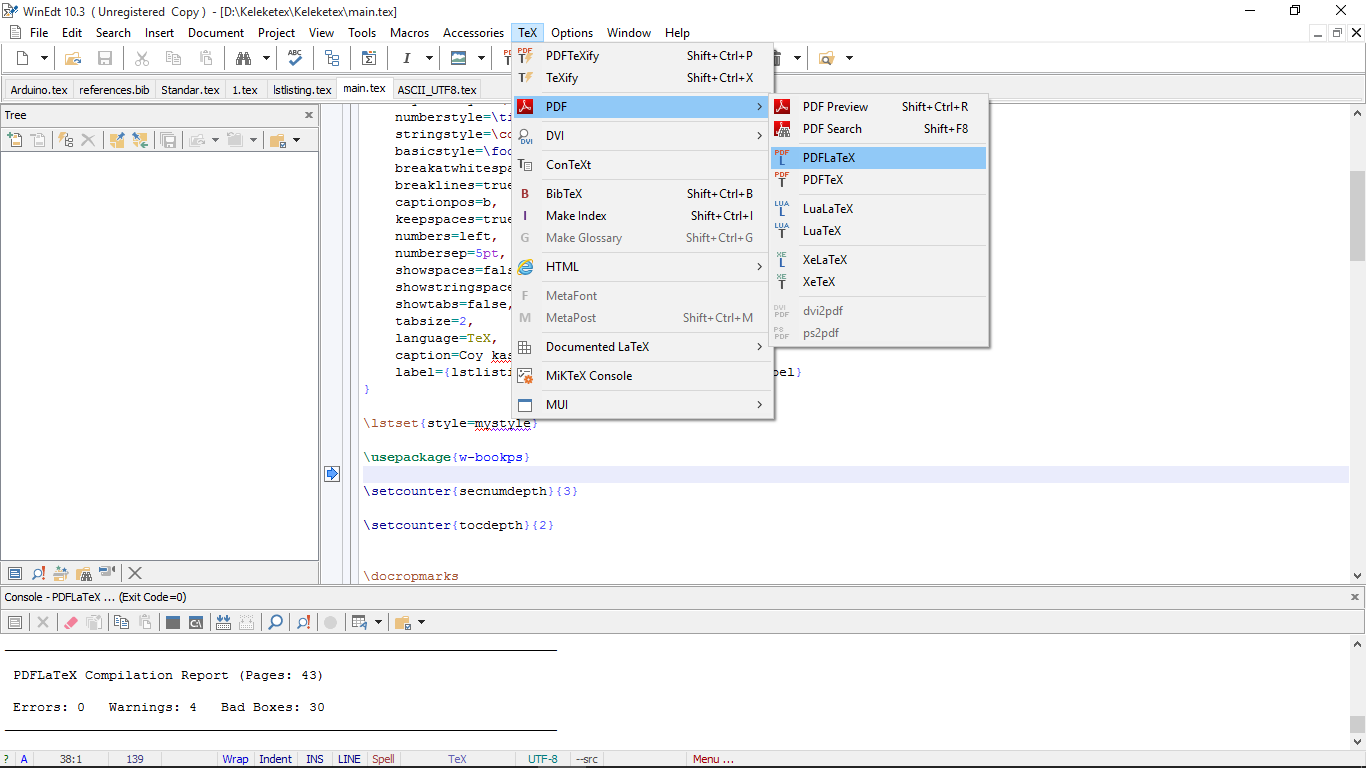
\includegraphics[width=.75\textwidth]{figures/pdflatex.png}
  \caption{Ini adalah Compile pdflatex}\label{fig:pdflatex}
\end{figure}
   \begin{figure}[!htbp]
  \centering
  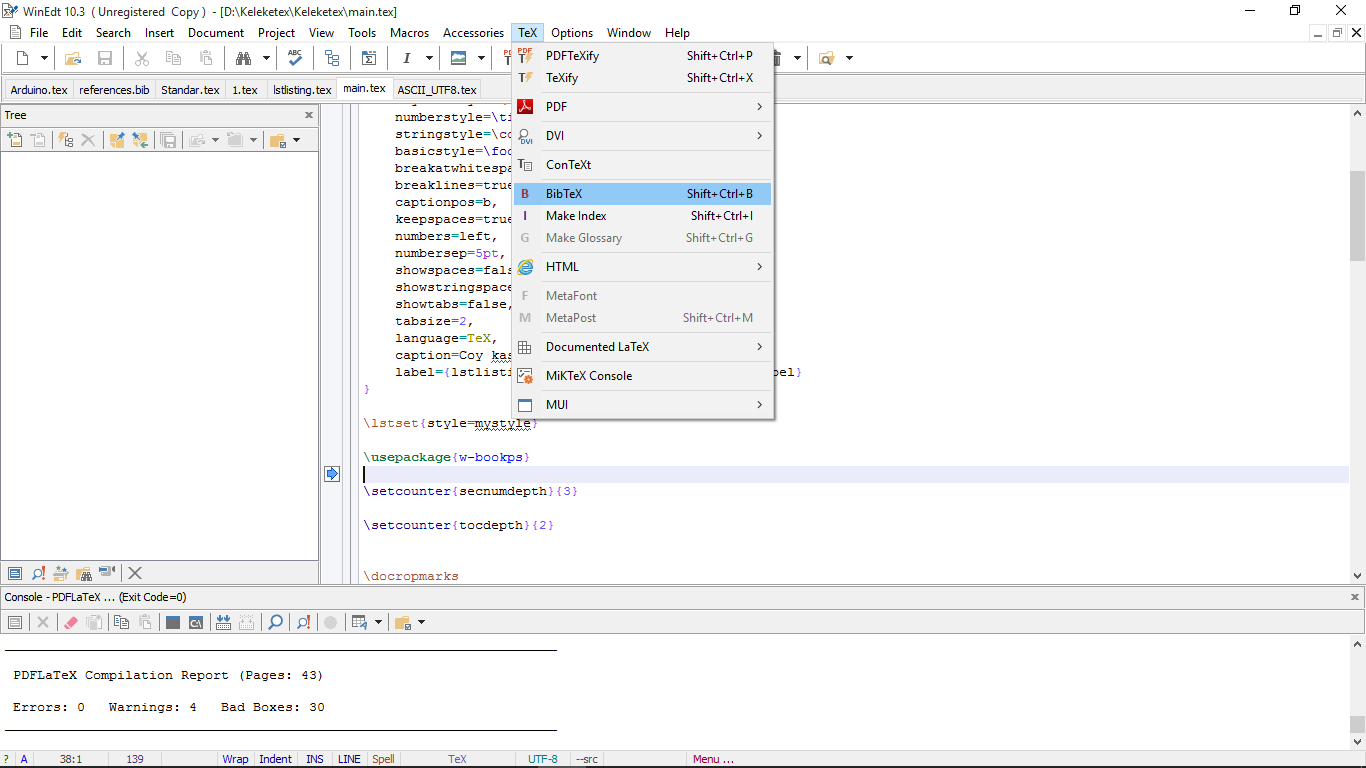
\includegraphics[width=.75\textwidth]{figures/bibtexx.png}
  \caption{Ini adalah Compile BibTex}\label{fig:bibtexx}
\end{figure}
\end{enumerate}



\chapter{Contoh Studi Kasus}
\section{Contoh studi kasus penggunaan aplikasi ini}
Smart Gudang merupakan sebuah aplikasi yang dirancang khusus untuk manajemen barang dimana cara kerja dari aplikasi ini dengan menunjukan scan barcode ke arah barang. Aplikasi ini ditujukkan bagi masyarakat yang memiliki usaha kecil yang terbatas biaya karena dilihat dari permasalahan yang ada dalam lingkup pergudangan bawah menengah masih banyak sekali kesulitan dalam hal pencatatan data sehingga tidak mengefisiensikan waktu. Dan dengan adanya aplikasi ini masyarakat yang memiliki usaha kecil tidak perlu merogoh banyak biaya unutk membeli alat scanner, cukup dengan menggunakan smartphone yang telah terinstall aplikasi scanner ini.

Tujuan
1.Mengefisiensikan waktu dengan mengubah teknologi tradisional menjadi teknologi modern
2.Mengganti device khusus scanner dengan android yang telah terintstall aplikasi smart Gudang
3.Mempermudah manajemen barang masuk dan barang keluar 

Manfaat
1.Mengefisiensi waktu dalam memanajemen barang masuk dan barang keluar 
2.Mengurangi biaya dalam pmenuhan alat device (alat scanner)
3.Masyarakat di permudah dalam memanajemen barang

\section{Manfaat Database}
Berikut beberapa manfaat dari menggunakan database yang bisa didapatkan jika bekerja dengan sistem database:
\begin{enumerate}
\item Tidak terjadinya redudansi Basis Data
\hfill \break
Database mampu meminimalkan terjadinya redudansi artinya redudansi sendiri itu merupakan terjadinya data-data ganda dalam berkas-berkas yang berbeda. 
\item Integritas Data Terjaga
\hfill \break
Database memastikan integritas data yang tinggi dimana database akan memastikan keakuratan,aksesbilitas, konsistensi dan juga kualitas tinggi pada suatu data.
\item Independensi Berbagai Data
\hfill \break
Database menjaga independensi data dimana orang lain tidak dapat merubah data meskipun data bisa diakses.
\item Kemudahan berbagai Data
\hfill \break
Menggunkan perangkat lunak database bisa digunakan untuk berbagi data atau informasi dengan sesa pengguna lainnya.
\item Menjaga Keamanan Data
Database menjamin keamanan suatu informasi data, dimana anda bisa meyisipkan kode akses untuk data-data tertentu yang tidak bisa diakses bersama.
\item Kemudahan Akses Data
\hfill \break
Dengan database bisa memudahkan untuk mengakses dan mendapatkan data karena semua data terorganisir dengan baik.
\end{enumerate}



\chapter{Contoh pemrograman sederhana Android Studio "Hello World"}
chapters/7

\chapter{Penggunaan Aplikasi untuk siapakah?}
chapters/8

\chapter{Apa perbedaan penggunaan Heroku dan Webhost?}
chapters/9

\chapter{Interfaces aplikasi}
chapters/10

\bibliographystyle{IEEEtran}
\bibliography{references}


\printindex
\end{document}

